% Isolated CPE manuscript using the downloaded Wiley New Journal Design class.
% Redirect the class-selected bibliography to the documented local AMA repair.
\let\CPEBibliographyStyle\bibliographystyle
\renewcommand{\bibliographystyle}[1]{\CPEBibliographyStyle{cpe-AMA}}
\documentclass[AMA,twocolumn]{USG}
\let\bibliographystyle\CPEBibliographyStyle
\usepackage{anyfontsize}
\usepackage{booktabs}
\usepackage{enumitem}
\usepackage{cpe-template-fixes}
\usepackage{xurl}
\microtypesetup{expansion=true}
\graphicspath{{./images/}{./figures/}}
\setlength{\emergencystretch}{2em}
\raggedbottom
\renewcommand{\topfraction}{0.90}
\renewcommand{\bottomfraction}{0.85}
\renewcommand{\textfraction}{0.08}
\renewcommand{\floatpagefraction}{0.80}
\renewcommand{\dbltopfraction}{0.90}
\renewcommand{\dblfloatpagefraction}{0.80}
\setcounter{dbltopnumber}{3}
\setcounter{topnumber}{3}
\setcounter{totalnumber}{4}
\articletype{RESEARCH ARTICLE}
\journal{Concurrency and Computation: Practice and Experience}
\received{}\revised{}\accepted{}
\volume{}\copyyear{}\startpage{1}\articledoi{}
\hypersetup{hidelinks,hypertexnames=false,
  pdftitle={Tie-Aware Characterization of Sparse-Index Gradient Accumulation for PyTorch CUDA Backpropagation},
  pdfauthor={Marko Mihajlovic}}
\begin{document}
\title{Tie-Aware Characterization of Sparse-Index Gradient Accumulation for PyTorch CUDA Backpropagation}
\author[1]{Marko Mihajlovic}[https://orcid.org/0009-0006-7979-0341]
\authormark{MIHAJLOVIC}
\titlemark{Tie-Aware Sparse-Index Gradient Accumulation}
\address[1]{\orgname{Singidunum University, }\orgaddress{\state{Belgrade, }\country{Serbia}}}
\corres{Marko Mihajlovic (\email{marko.mihajlovic.23@singimail.rs})}
\keywords{sparse gradients | indexed accumulation | backpropagation | PyTorch | CUDA | embedding backward | performance characterization}

\abstract[ABSTRACT]{
Sparse-index gradient accumulation is a recurring operation in embedding-heavy and sparse-feature training workloads, where repeated indices route multiple gradient contributions to shared parameter rows during backpropagation. Although PyTorch exposes several semantically related CUDA paths for this pattern, API-level similarity does not imply interchangeable execution behavior. This paper characterizes three standard paths, \texttt{index\_\allowbreak add}, \texttt{scatter\_\allowbreak add}, and \texttt{Embedding.\allowbreak backward}, using correctness-gated benchmarks, matched sparse-index workload grids, CUDA-event timing, profiler inspection, threshold-sensitivity checks, descriptive bootstrap intervals, regret analysis, and a controlled backward-style proxy.

Across two distinct GPU/software stacks, the fastest path depends on workload shape, timing scope, and execution stack. The matched isolated benchmark and the backward-style proxy do not yield the same ranking, showing that isolated accumulation results should not be transferred mechanically to broader backpropagation-style computation. Profiler summaries further show that the three paths use distinct CUDA execution-path compositions, including direct accumulation kernels for the tensor APIs and a multi-kernel embedding backward path with sorting or segmentation-related components. These findings make sparse-index gradient accumulation a systems-level backpropagation concern rather than a purely semantic API choice.

The analysis also shows why a tie-aware interpretation is needed. Practical-margin threshold checks and winner maps reveal workload regions with decisive winners and regions dominated by near-ties, while regret analysis shows that static API selection can still be costly. The lowest-mean-regret static choice varies by stack and scope, and the smallest observed worst-case static regret still reaches 145.0\%, precluding a safe universal default. The practical output is therefore not a universal ranking of \texttt{index\_\allowbreak add}, \texttt{scatter\_\allowbreak add}, and \texttt{Embedding.\allowbreak backward}, but a measurement-backed, tie-aware selection protocol: measure candidate paths under the target sparse workload and execution stack, treat small differences as practical ties, validate isolated rankings against a broader backward-style scope when relevant, and use profiler evidence to inspect execution-path divergence.
}

\maketitle
\section{Introduction}

Modern AI training workloads are not composed only of dense matrix multiplication, convolution, or attention kernels. Many practical models also contain sparse or irregular components whose performance is shaped by index distributions, memory access patterns, and reduction behavior. This is especially visible in recommendation and sparse-feature models, where large embedding tables are used to represent categorical identifiers and where training efficiency depends on both dense neural-network computation and memory-intensive embedding operations \citep{gupta2020architectural}. Recent work on large-scale embedding optimization further shows that embedding access patterns, repeated indices, and gradient processing remain important systems-level concerns in recommendation-model training \citep{liu2024embark}.

A central operation in such workloads is sparse-index gradient accumulation during backpropagation. In the forward pass, indexed operations such as embedding lookup gather rows from a parameter table. In the backward pass, gradients associated with those indexed rows must be routed back and accumulated into the corresponding parameter-gradient structure. When the same index appears multiple times in a batch, several gradient contributions target the same destination row. This creates an indexed aggregation problem rather than a purely dense tensor operation. The cost of this aggregation can depend on the number of rows, number of indices, feature dimension, index skew, duplicate-index frequency, memory layout, and the CUDA execution path selected by the framework.

From a parallel-computing perspective, these operations are instances of irregular indexed reduction: many source vectors update a smaller set of destination rows, and duplicate or skewed indices create contention, ordering, and memory-access effects. This makes stack-sensitive performance behavior a performance-portability concern for high-level GPU tensor APIs, beyond API convenience in machine-learning code.

We use PyTorch as the experimental framework \citep{paszke2019pytorch}. The compared paths are direct indexed accumulation through \texttt{index\_\allowbreak add} and \texttt{scatter\_\allowbreak add}, and gradient accumulation through \texttt{Embedding.\allowbreak backward}. Our workload construction makes their dense row-gradient outputs comparable; it does not assume identical API contracts or internal execution paths. The operator names identify the implementations evaluated here, rather than implying interchangeable kernel behavior.

CUDA kernel execution is asynchronous with respect to the host, making synchronization-aware timing essential \citep{nvidia2026cudaguide}. Repeated measurements, variability reporting, and reproducible experimental conditions are also central to scientific performance comparisons \citep{hoefler2015benchmarking}. We therefore separate unprofiled CUDA-event timing from profiler-based execution-path attribution and validate numerical outputs before accepting timing rows.

Prior work develops sparse GPU kernels \citep{gale2020sparse} and optimizes GPU recommendation training and embedding-gradient processing \citep{mudigere2022neo,liu2024embark}. These studies connect performance to workload structure and execution strategy. Our question concerns the high-level framework interface: how do standard PyTorch CUDA paths compare under matched sparse-index gradient accumulation workloads, and how should practical ties inform implementation choice?

This paper addresses that question through a controlled empirical study of sparse-index gradient accumulation during backpropagation-style computation. The study evaluates standard PyTorch CUDA paths rather than custom CUDA kernels. It first calibrates the benchmark protocol and validation rules, then performs a matched grid-level timing comparison, uses representative profiler runs to relate timing behavior to CUDA execution paths, and finally adds a small training-step proxy to examine whether isolated sparse-index accumulation behavior remains visible in a broader backward-style computation. The main systems contribution is a reproducible performance characterization and measurement-backed interpretation framework for workload-, scope-, and stack-dependent behavior, culminating in a tie-aware selection protocol.

The paper makes five contributions:
\begin{itemize}
\item A correctness-gated, reproducible comparison of three standard PyTorch CUDA sparse-index accumulation paths: \texttt{index\_\allowbreak add}, \texttt{scatter\_\allowbreak add}, and \texttt{Embedding.\allowbreak backward}.
\item Evidence of workload-, scope-, and stack-dependent behavior across the GTX1650Ti and hosted Colab T4 stacks, using matched isolated benchmarks and a backward-style proxy.
\item Profiler-backed evidence of distinct CUDA execution-path compositions, interpreted at the stack level rather than as isolated hardware causality.
\item Threshold-sensitivity and descriptive bootstrap checks, winner maps, and regret/minimax analyses that contextualize practical ties and quantify static-selection costs.
\item A measurement-backed, tie-aware selection protocol for comparing candidate paths under the target workload and execution stack.
\end{itemize}

The rest of the paper is organized as follows. Section~\ref{sec:background-related-work} reviews sparse operations in AI training, embedding-heavy workloads, indexed accumulation APIs, CUDA execution behavior, and related profiling methodology. Section~\ref{sec:methodology} describes the benchmark scope, workload design, correctness validation, timing methodology, profiling methodology, and cross-environment comparison. Section~\ref{sec:results-analysis} presents the calibrated benchmark results, matched Phase 2 timing evidence, representative Phase 3 profiler results, the Phase 4 training-step proxy, and result-level discussion. Section~\ref{sec:general-discussion} discusses significance, practical implications, limitations, generalizability, and future work. Section~\ref{sec:conclusion} concludes the paper.
\section{Background and Related Work}
\label{sec:background-related-work}

Recommendation models combine dense neural computation with embedding tables for sparse categorical features. Gupta et al. characterize the embedding and memory-access demands of production recommendation workloads \citep{gupta2020architectural}. Acun et al. examine training efficiency at scale, connecting model configuration and data placement to system performance \citep{acun2021training}. These works motivate embedding-heavy workloads without identifying the relative costs of the three framework paths studied here.

GPU embedding systems address a broader optimization problem. Neo combines software and hardware techniques, including embedding-operator optimization and kernel fusion, for scalable recommendation training \citep{mudigere2022neo}. HugeCTR provides GPU-accelerated training and inference infrastructure for recommendation models \citep{wang2022hugectr}. Embedding-table capacity and memory traffic are separate constraints: FLECHE studies GPU embedding caching, while ScratchPipe addresses embedding working sets and CPU/GPU traffic during training \citep{xie2022fleche,kwon2022scratchpipe}. These systems establish the importance of embedding computation and memory management; they are not baselines for our single-GPU accumulation comparison.

Sparse and irregular GPU computation provides complementary context. Gale et al. study sparse deep-learning kernel optimization \citep{gale2020sparse}. GE-SpMM examines sparse matrix multiplication for graph neural networks, where data reuse and irregular memory access affect execution efficiency \citep{huang2020gespmm}. Gunrock's data-centric graph processing addresses irregular work distribution through frontier-based GPU execution \citep{wang2016gunrock}. These workloads motivate attention to memory access and load balance, but sparse matrix multiplication and graph traversal are not equivalent to embedding-gradient accumulation.

Sorting and scan primitives explain one family of indexed-reduction strategies. GPU radix sorting groups equal keys \citep{satish2009sorting}, and scan and segmented scan provide building blocks for operations on grouped irregular data \citep{sengupta2007scan}. Thrust exposes sorting, scan, and reduction through a high-level interface interoperable with CUDA \citep{bell2011thrust}. Conceptually, a sorting-based path proceeds from indices through grouping or sorting, duplicate-key aggregation or segmented reduction, and a sparse update of the referenced rows.

Earlier GPU work examines contention and order-dependent summation when concurrent floating-point atomic updates concentrate on the same destination, motivating reorganized accumulation schemes \citep{defour2015reproducible}. EMBark connects these primitives directly to embedding training. It addresses skewed accesses and load imbalance through partial-gradient aggregation, including sorting gradients by category/index and segmented reduction to reduce expensive atomic accumulation \citep{liu2024embark}. This is closely related algorithmic context for the sort, scan, and accumulation components identified by our profiler summaries. Our study characterizes existing PyTorch paths; it does not implement an additional sorted-aggregation path or directly compare primitive libraries and specialized embedding systems.

At the programming-model level, CUDA supports atomic updates and asynchronous device execution \citep{nvidia2026cudaguide}. Floating-point non-associativity means that different parallel addition orders can yield numerically different results; GPU/HPC work studies this reproducibility problem and deterministic alternatives \citep{shanmugavelu2024nonassociativity}. This motivates tolerance-based correctness checks where reduction order may vary. At the experimental level, Hoefler and Belli emphasize repeated measurements, variability, and reproducible performance reporting \citep{hoefler2015benchmarking}. Our methodology combines these concerns through correctness-gated timing, explicit timing scopes, and separate diagnostic profiling. The practical-margin rule is a descriptive interpretation choice in this study, not a statistical test prescribed by those sources.

The contribution is a controlled characterization at the PyTorch API boundary. By matching sparse-index workloads across standard paths and relating timings to execution-path evidence, the study examines workload-, scope-, and stack-dependent behavior and develops measurement-backed, tie-aware selection guidance. It complements system-level embedding optimization without claiming a new GPU primitive or production-training speedup.

\section{Methodology}
\label{sec:methodology}

\subsection{Study Scope}

This study investigates sparse-index gradient accumulation patterns that arise during the backpropagation phase of AI model training. The focus is on workloads in which many indexed source vectors contribute to a dense gradient-like output, a pattern that is common in embedding tables, recommender-style models, negative sampling, graph workloads, and other training settings where sparse index references are accumulated during the backward pass.

The experiments are implemented in PyTorch \citep{paszke2019pytorch} and scoped to standard CUDA execution paths rather than custom CUDA kernels. The goal is not to design a new accumulation primitive, but to characterize how widely available PyTorch APIs behave under controlled sparse-index accumulation workloads. In particular, the experiments examine whether API-level alternatives that express similar accumulation-style computations can exhibit different timing behavior and different CUDA execution paths.

The study does not benchmark full production model training, end-to-end training throughput, dense matrix multiplication, convolution, attention, optimizer performance, data loading, or distributed training. These components are outside the scope because they would introduce additional sources of variation that are not necessary for isolating the sparse-index accumulation behavior studied here. Instead, the experimental design separates a grid-level timing phase, a representative profiling phase, and a small training-step proxy. The grid-level phase provides the main matched timing evidence, the profiling phase provides execution-path attribution for selected representative cases, and the proxy tests whether the observed sparse-index accumulation behavior remains visible when embedded in a controlled backward-style computation.

\subsection{Benchmarked Operations}

The comparison centers on three PyTorch CUDA operations or operation paths:

\begin{itemize}[leftmargin=*]
    \item \texttt{index\_\allowbreak add}, which accumulates source rows into a dense output according to an index tensor;
    \item \texttt{scatter\_\allowbreak add}, which expresses an indexed accumulation pattern through scatter-style updates;
    \item \texttt{Embedding.\allowbreak backward}, which represents the backward path of a PyTorch embedding table and therefore provides a realistic training-related sparse-gradient accumulation path.
\end{itemize}

These operations are conceptually related because each can be used to represent sparse-index accumulation into a dense gradient-like tensor under controlled workload construction. However, the study does not assume that they are universally equivalent in all PyTorch contexts or all mathematical formulations. Instead, they are compared under matched accumulation-style workloads in which the input shapes, index distributions, and output dimensions are controlled.

The inclusion of \texttt{Embedding.\allowbreak backward} is important because embedding tables are a common source of sparse gradient accumulation during backpropagation. Unlike the direct accumulation APIs, the embedding backward path may involve specialized internal kernels and additional framework-level logic. Comparing it with \texttt{index\_\allowbreak add} and \texttt{scatter\_\allowbreak add} therefore helps distinguish API-level similarity from actual CUDA execution behavior.

\subsection{Workload Design}

Workloads are parameterized by the number of output rows, the number of indexed source entries, the feature dimension, and the distribution of index values. The main workload parameters are:

\begin{itemize}[leftmargin=*]
    \item \texttt{rows}: the number of rows in the dense output or embedding table;
    \item \texttt{indices}: the number of indexed source entries accumulated during the operation;
    \item \texttt{dim}: the feature dimension of each row;
    \item \texttt{distribution}: the statistical distribution used to generate index references;
    \item \texttt{workload\_\allowbreak draw}: the workload draw identifier used to construct matched cases;
    \item \texttt{zipf\_\allowbreak mode}: the mode used for Zipf-distributed workloads;
    \item \texttt{row\_\allowbreak layout}: the layout of rows in the generated workload;
    \item \texttt{index\_\allowbreak order}: the order of generated indices;
    \item \texttt{cache\_\allowbreak mode}: whether the workload is evaluated under the selected cache condition.
\end{itemize}

The workload distributions include uniform, Zipf, and hotspot-style index patterns. Uniform workloads provide a baseline in which index references are more evenly distributed across rows. Zipf and hotspot workloads introduce skew, duplicate references, and hot rows. These skewed cases are important because duplicate indices can change the cost of accumulation and can expose differences between accumulation implementations.

The broader timing phase evaluates matched configurations across a larger workload grid. The profiling phase uses a smaller set of representative cases selected to expose the CUDA execution paths underlying the observed API behavior. This separation avoids relying on profiler-instrumented runs as the primary timing evidence while still allowing the study to inspect representative kernel-level composition.

\subsection{Correctness Validation}

Correctness validation is performed before timing or profiling results are accepted into the analysis. This is necessary because timing comparisons are meaningful only when the operations compute the intended accumulation result under the same workload configuration.

For each accepted configuration, the benchmark checks that the compared operation produces numerically valid output relative to the reference accumulation behavior used by the experiment. Rows with failed correctness checks or failed execution status are excluded from paired winner claims. This rule applies both to the broader timing phase and to the representative profiling phase.

The correctness procedure is especially important for sparse-index workloads because repeated indices, skewed distributions, and different execution paths may change floating-point accumulation order. Since floating-point addition is non-associative, such changes need not preserve bitwise identity \citep{shanmugavelu2024nonassociativity}. Validation therefore checks computational equivalence within explicit numerical tolerances before timing rows are accepted.

\subsection{Timing Methodology}

The primary timing evidence comes from repeated CUDA-event measurements over matched workload configurations. Synchronization-aware timing accounts for asynchronous CUDA execution \citep{nvidia2026cudaguide}, while repeated observations and attention to variability address scientific benchmarking concerns \citep{hoefler2015benchmarking}. Studies of production HPC systems further report performance variation among nominally identical GPUs \citep{sinha2022variability}, reinforcing the need to report the tested hardware/software stack and avoid overgeneralizing numerical results. For each configuration, the selected operations are compared within the same workload setting. The timing analysis uses median latency as the main summary statistic, because medians are less sensitive to occasional runtime outliers than single measurements or means alone.

A practical margin threshold is used to distinguish decisive timing differences from near-ties. Specifically, when the runner-up operation is more than 5\% slower than the fastest operation for a matched configuration, the fastest operation is treated as the practical winner for that case. If the margin does not exceed this threshold, the case is retained as a practical near-tie. The 5\% rule is a descriptive decision threshold, not a test of statistical significance.

The broader matched timing phase is the main source of grid-level performance evidence. The representative profiling phase also records event timings for the selected cases, but those timings are used primarily to relate profiled cases to the broader benchmark behavior. They are not treated as a replacement for the broader timing grid because the profiling subset is smaller and uses a fixed representative design.

The timing methodology distinguishes between direct operation timing and profiler-derived quantities. CUDA-event medians are used for operation-level timing comparisons, while profiler-derived CUDA totals are used for attribution and diagnostic interpretation. These two measurement sources are not interchangeable because profiling introduces instrumentation, synchronization, and event collection overhead.

\subsection{Profiling Methodology}

The profiling phase identifies the CUDA execution paths associated with the selected PyTorch APIs. For each case--operation pair, the analysis records execution status, timing summaries, case-level winners and runners-up, timing-stability flags, host-overhead warnings, and kernel-category shares. Full profiler events and summaries of the leading CUDA events provide complementary levels of attribution detail.

Full CUDA event files are preferred over top-event summaries when computing kernel-category shares. User annotations and enclosing profiling ranges are excluded from category-share calculations so that the resulting summaries reflect CUDA device work rather than inclusive annotation ranges. When only top-event summaries are available, the analysis treats them as truncated attribution evidence rather than full-profile composition.

The profiler events are grouped into conservative name-based categories. The categories used for interpretation are:

\begin{itemize}[leftmargin=*]
    \item \texttt{index\_\allowbreak add\_\allowbreak accumulate}, for CUDA kernels associated with indexed reduction through the \texttt{index\_\allowbreak add} path;
    \item \texttt{scatter\_\allowbreak add\_\allowbreak accumulate}, for CUDA kernels associated with scatter/gather reduction paths;
    \item \texttt{embedding\_\allowbreak accumulate}, for embedding backward accumulation kernels such as gradient-weight computation and scatter-style accumulation inside the embedding backward path;
    \item \texttt{sort\_\allowbreak scan\_\allowbreak unique}, for sort, scan, and unique-related kernels that appear in the embedding backward path;
    \item \texttt{zero\_\allowbreak fill\_\allowbreak memset}, for initialization and zero-fill kernels;
    \item \texttt{arange\_\allowbreak index\_\allowbreak setup}, for index setup kernels such as range construction;
    \item \texttt{other}, for CUDA events not captured by the preceding categories.
\end{itemize}

These categories are used for execution-path attribution, not for proving low-level hardware causality. They are based on observed kernel and operator names, and therefore depend on the PyTorch and CUDA software stack used in each environment. The category summaries are intended to show whether the three PyTorch APIs exercise distinct CUDA paths under the profiled workloads.

The profiling phase also computes a GPU-busy proxy by comparing profiler-derived CUDA kernel time with the unprofiled CUDA-event timing for the same case. This proxy is used only as a warning signal for possible host overhead. It is not a hardware utilization counter and is not interpreted as a direct measurement of GPU occupancy or saturation.

\subsection{Training-Step Proxy Methodology}

To complement the isolated accumulation measurements, the study includes a small training-step proxy. It provides a controlled backward-style workload in which the accumulation path is embedded in lookup, grouped mean pooling, a scalar prediction head, mean-squared error, and backward propagation.

The proxy compares three variants. The \texttt{embedding\_\allowbreak backward\_\allowbreak proxy} variant uses native dense Embedding backward. The \texttt{index\_\allowbreak add\_\allowbreak proxy} and \texttt{scatter\_\allowbreak add\_\allowbreak proxy} variants use custom autograd lookup nodes that allocate a dense zero gradient and accumulate row gradients with the corresponding PyTorch API. The variants share the same generated inputs, pooling structure, prediction head, and loss computation.

Two timing scopes are recorded. The \texttt{proxy\_\allowbreak step} scope measures the full synthetic step, including lookup, pooling, prediction, loss, and gradients for the table, head, and bias. The \texttt{accumulation\_\allowbreak region} scope separately replays backward through a retained lookup graph with fixed upstream gradients. This second scope is diagnostic: it includes autograd dispatch, dense gradient allocation and zeroing, and accumulation, but it is not an exact decomposition of the proxy step and is not subtracted from total-step latency.

The proxy uses the same practical-margin rule as the other timing analyses. A variant is counted as a winner only when the runner-up median is strictly more than 5\% slower; otherwise the observation is classified as a practical tie. The proxy is evaluated with five seeds per environment and 24 configurations per seed, giving 120 seed--configuration observations per environment.

\subsection{Cross-Environment Comparison}

The study compares two distinct GPU/software stacks: a GTX1650Ti stack and a hosted Colab T4 stack. These stacks differ not only in GPU model, but also in operating system, runtime conditions, PyTorch version, CUDA version, and hosted execution context. Therefore, the comparison is interpreted as a stack-level comparison rather than an isolated hardware-causal experiment.

Table~\ref{tab:environment-stack-summary} summarizes the hardware and software stacks used for the reported measurements.

% Verified against saved Phase 2 confirmation, Phase 3 v2, and Phase 4 metadata.
% Full platforms: Windows-10-10.0.19045-SP0;
% Linux-6.6.122+-x86_64-with-glibc2.39. OS labels below are shortened for display.
\begin{table*}[t]
\centering\fontsize{9}{11}\selectfont
\caption{Hardware and software stacks used in the reported experiments. The T4 repeat is a repeat run on the hosted T4 stack, not a separate independent environment.}
\label{tab:environment-stack-summary}
\setlength{\tabcolsep}{3pt}
\renewcommand{\arraystretch}{1.12}
\begin{tabularx}{\linewidth}{@{}>{\raggedright\arraybackslash}p{1.9cm}>{\raggedright\arraybackslash}p{3.0cm}>{\raggedright\arraybackslash}p{3.6cm}ll>{\raggedright\arraybackslash}X@{}}
\toprule
Stack & GPU & OS/runtime & PyTorch & CUDA & Role \\
\midrule
GTX1650Ti & NVIDIA GeForce GTX 1650 Ti & Windows 10.0.19045 & 2.13.0+cu126 & 12.6 & Local workstation \\
Colab T4 & Tesla T4 & Linux 6.6.122+ / Colab & 2.11.0+cu130 & 13.0 & Hosted stack \\
\bottomrule
\end{tabularx}
\end{table*}


Phase~2 includes a repeat run of the T4 stack, not a third independent environment. The training-step proxy uses the same stack-level interpretation, with GTX1650Ti and T4 results paired by seed and configuration where possible.

The cross-environment analysis is performed in two stages. First, the broader matched timing analysis compares winner counts, practical-margin winners, and relative speedups across the matched workload grid. Second, the representative profiling analysis compares selected cases across the two environments and relates them back to the matched timing grid.

The profiling comparison records case-level winners, margins, timing-stability flags, host-overhead warnings, and index-hash pairing status. A separate join links the profiled cases back to the broader Phase~2 grid. Evidence criteria distinguish decisive, stable, exactly paired reversals from near-ties or cases affected by host-overhead warnings.

Workload pairing is checked through parameter matching and index hashes where available. Matching index hashes provide stronger evidence that the same index draw is being compared across environments. Source tensor hashes may differ across environments due to random number generation and software-stack differences, so source-hash mismatches are treated as informational rather than automatic failures.

\subsection{Validity Boundaries and Reproducibility}

The profiler phase uses representative cases for execution-path attribution, while Phase~2 supplies the main grid-level timing evidence. The comparison concerns two GPU/software stacks whose GPU model, operating system, PyTorch version, CUDA version, and runtime conditions vary together. The synthetic proxy does not measure production training throughput, optimizer behavior, or distributed execution, and custom CUDA alternatives are outside the study scope.

These boundaries are revisited in the Discussion, where the regret analysis and tie-aware protocol are also limited to descriptive interpretation over saved observations.

\noindent\textbf{Reproducibility.}

The benchmark harness, aggregation scripts, and generated result artifacts are maintained in a public repository at \url{https://github.com/mihajlov39547/sparse-index-gradient}. The reported analyses use fixed seeds, saved raw and summary CSV artifacts, metadata files recording PyTorch and CUDA versions, and validation outputs for each accepted run. The measured hardware and software stacks are summarized in Table~\ref{tab:environment-stack-summary}.

\section{Results and Analysis}
\label{sec:results-analysis}

This section presents the experimental evidence in the same order in which the benchmark design was developed and validated. The first phase establishes the baseline behavior of the benchmark and verifies the methodological assumptions needed for fair comparison. The second phase provides the main matched grid-level timing evidence across the selected PyTorch CUDA accumulation paths. The third phase complements the timing results with profiler evidence for representative cases, allowing the observed performance differences to be related to the CUDA execution paths used by each API.

The analysis therefore separates three roles. Phase 1 is treated as a calibration and validation phase, because its purpose is to justify the final benchmark protocol rather than to provide the main paper-level performance claim. Phase 2 is treated as the primary timing phase, because it compares the selected operations across a matched workload grid. Phase 3 is treated as the attribution phase, because it explains selected Phase 2 patterns through CUDA profiler evidence. This separation is important because the study does not rely on a single timing table or a single profiler run; instead, the final interpretation combines protocol validation, matched timing, and representative execution-path analysis.

\subsection{Phase 1 Baseline Calibration and Methodological Checks}

Phase~1 calibrated the final benchmark protocol rather than supporting paper-level performance claims. Preliminary runs established a dense-gradient accumulation scope that includes output allocation or zero initialization where required by the operation design. They also confirmed that \texttt{Embedding.\allowbreak backward} should be treated as a standard framework path with its own dispatch behavior, rather than a syntactic alias for the direct accumulation APIs.

The calibration phase fixed the acceptance and interpretation rules used later. Tolerance-based correctness validation precedes acceptance of timing rows because repeated indices and different CUDA paths can change floating-point accumulation order. Median CUDA-event latency summarizes each timing distribution; a winner is decisive only when the runner-up is more than 5\% slower. Smaller differences remain practical ties.

Phase~1 also motivated varying uniform, Zipf, and hotspot-style index distributions alongside workload shape. The final protocol combines matched workloads, correctness-gated rows, median timing, and practical-margin classification, while separating grid-level timing evidence from profiler-based attribution. The main performance evidence begins with Phase~2.

\subsection{Matched Phase 2 Benchmark Results}

The matched Phase 2 benchmark provides the main grid-level evidence for the study. In this phase, the three selected PyTorch accumulation paths were compared under shared workload configurations, using the same rows, index counts, feature dimensions, distribution types, layout settings, and cache conditions within each matched case. The purpose of this phase was to determine whether the fastest API path is stable across environments or whether it changes with the workload and software/hardware stack.

Table~\ref{tab:phase2-winner-counts} summarizes the practical-margin winner counts across the matched Phase 2 grid. The GTX1650Ti stack favored \texttt{embedding} most often, with 96 decisive wins out of 162 matched configurations. The same environment selected \texttt{index\_\allowbreak add} in 60 configurations, while \texttt{scatter\_\allowbreak add} did not obtain a decisive win under the practical-margin rule. Six configurations were classified as ties. In contrast, the T4 stack favored \texttt{scatter\_\allowbreak add} most often, with 92 decisive wins out of 162 configurations. The repeated T4 run reproduced the same qualitative pattern, with \texttt{scatter\_\allowbreak add} selected in 93 out of 162 configurations.

% Source summary: sparse-gradient/phase2_analysis_v2/ and matched Phase 2 analysis.
\begin{table*}[t]
\centering
\fontsize{9}{11}\selectfont
\caption{Matched Phase 2 winner counts for the three primary accumulation paths under the 5\% practical-margin rule.}
\label{tab:phase2-winner-counts}
\setlength{\tabcolsep}{3pt}
\renewcommand{\arraystretch}{1.12}
\begin{tabularx}{\linewidth}{@{}lrrrr>{\raggedright\arraybackslash}X>{\raggedright\arraybackslash}X@{}}
\toprule
Environment & \texttt{index\_add} & \texttt{scatter\_add} & \texttt{embedding} & Tie & Total matched configurations & Most frequent decisive API \\
\midrule
GTX1650Ti & 60 & 0 & 96 & 6 & 162 & \texttt{embedding} \\
T4 & 5 & 92 & 25 & 40 & 162 & \texttt{scatter\_add} \\
T4\_repeat & 1 & 93 & 27 & 41 & 162 & \texttt{scatter\_add} \\
\bottomrule
\end{tabularx}
\end{table*}


The Phase~2 results show a change in the most frequently favored path across the measured stacks. The GTX1650Ti stack most often favors the embedding backward path, whereas the T4 stack and its repeat run most often favor the scatter-add path. This difference is not interpreted as an isolated GPU-hardware effect, because the environments differ in GPU model, operating system, PyTorch version, CUDA version, and hosted execution conditions. Instead, the result motivates a stack-level interpretation: the relative cost of the available PyTorch CUDA paths depends on the combination of workload structure and execution environment.

The practical-margin rule is important for interpreting these counts. Configurations in which the fastest and runner-up operations differ by no more than the selected 5\% threshold are retained as near-ties rather than treated as decisive evidence. This prevents small timing differences from being overinterpreted as meaningful API-level superiority. Consequently, the Phase 2 result should be read as a matched practical-performance characterization, not as a statistical proof of an API ordering that applies across workloads and stacks.

\subsection{Representative Phase 3 Profiling Results}

Phase 3 complements the Phase 2 timing grid by profiling a representative subset of six workload cases. The purpose of this phase is not to replace the broader timing evidence, but to inspect the CUDA execution paths associated with the selected PyTorch APIs. Each representative case is evaluated for \texttt{index\_\allowbreak add}, \texttt{scatter\_\allowbreak add}, and \texttt{Embedding.\allowbreak backward}, resulting in 18 profiled case-operation rows per environment.

The profiling outputs passed the basic execution and correctness checks in both environments. Each environment produced 18 successful case-operation rows, with no failed execution status and no correctness failures. CUDA kernel attribution was available for all 18 profiled rows in both environments. The T4 environment contained one host-overhead warning, associated with the \texttt{embedding} operation in case04; this case is therefore interpreted cautiously when making GPU-clean attribution claims.

Figure~\ref{fig:phase3-median-ms} shows the representative Phase 3 event-timing medians by case and operation. These values are useful for relating the profiled subset to the broader timing behavior, but they are not treated as a replacement for the matched Phase 2 grid. The profiled subset uses a smaller number of cases and is primarily designed for attribution rather than grid-level performance counting.

\begin{figure*}[t]
\centering
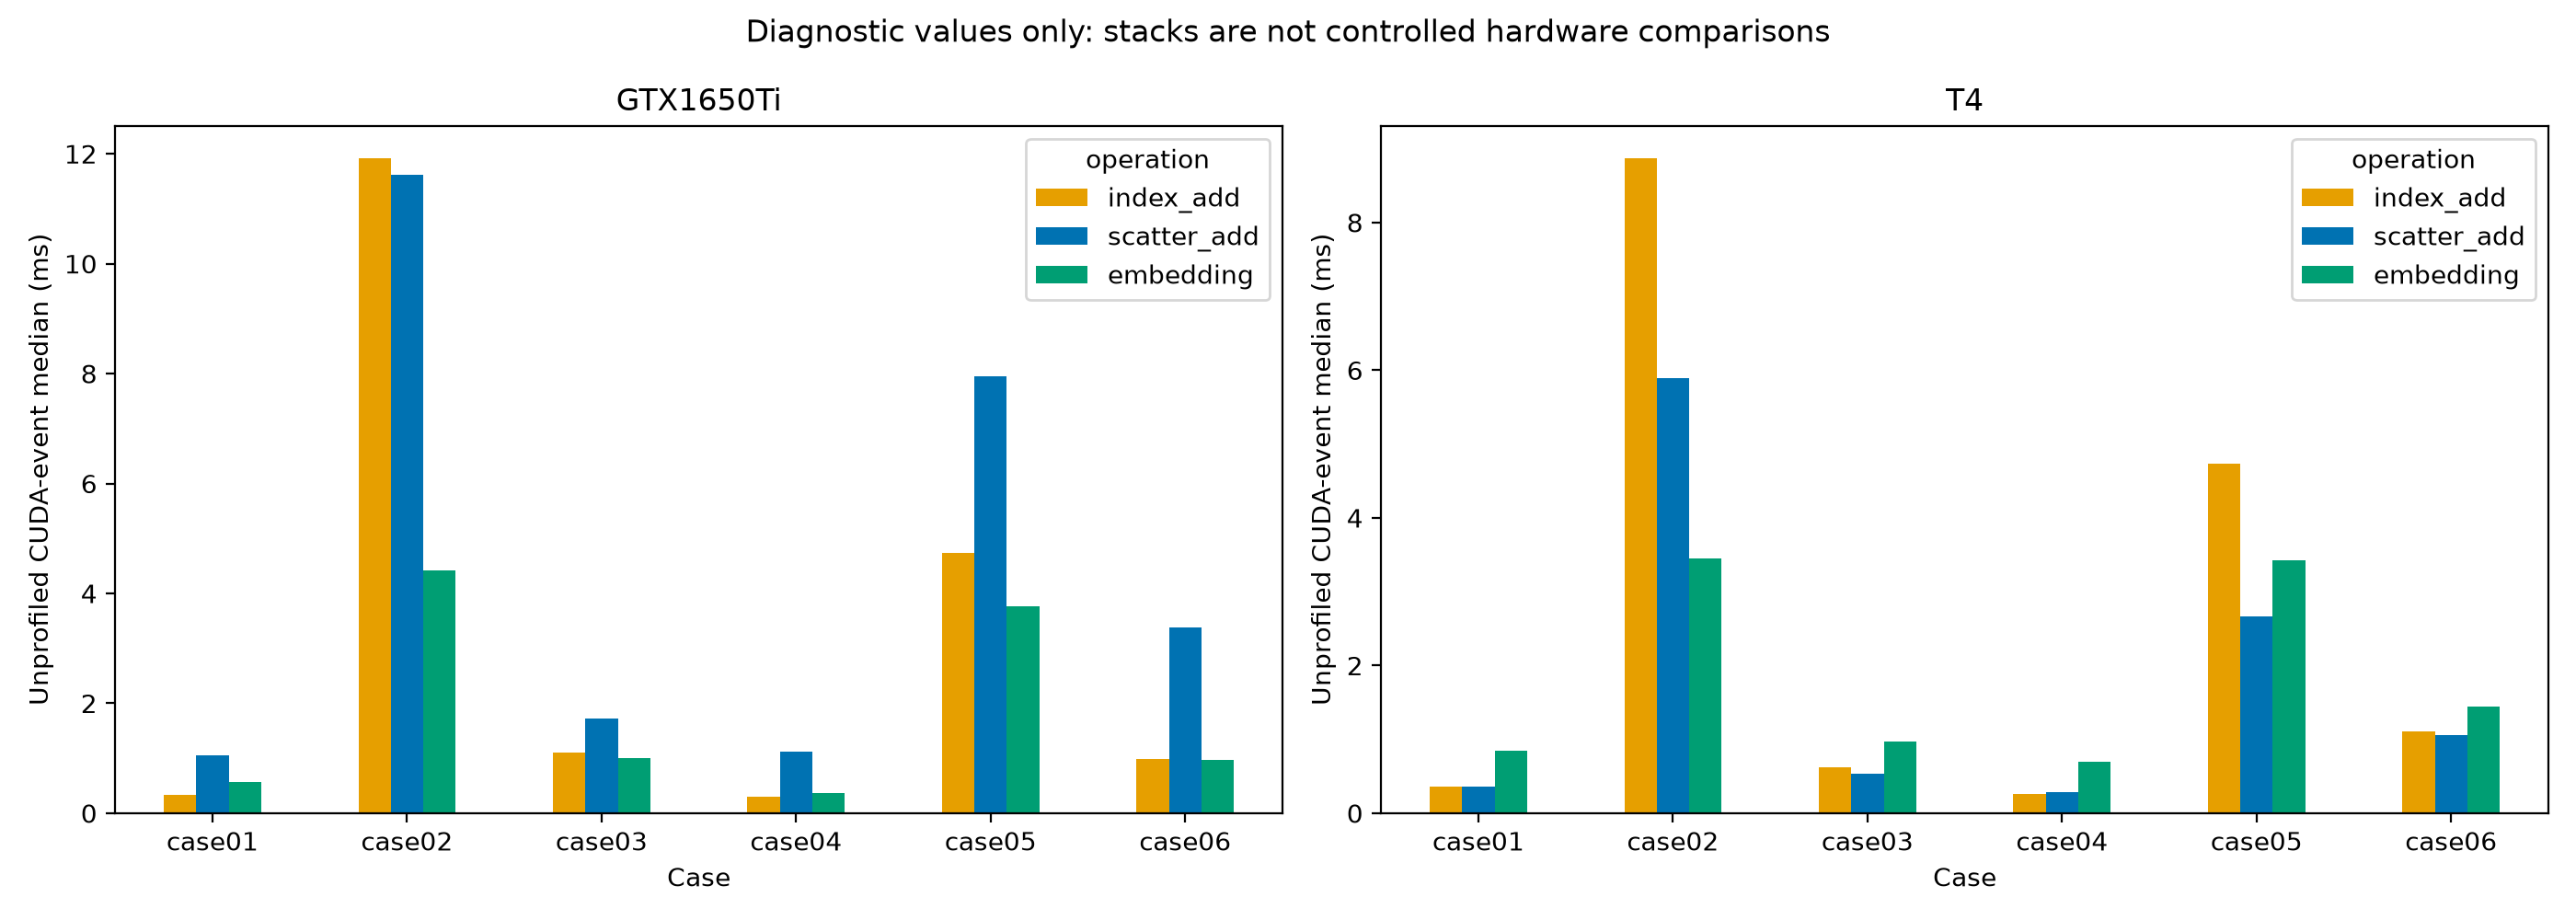
\includegraphics[width=0.95\linewidth]{figures/phase3_median_ms_by_case_operation.png}
\caption{Phase 3 median CUDA-event timing by representative case and operation. These timings describe the profiled subset and are interpreted together with the broader matched Phase 2 grid.}
\label{fig:phase3-median-ms}
\end{figure*}

Figure~\ref{fig:phase3-gpu-busy} summarizes the profiler-derived GPU-busy proxy. The proxy is used only as a warning signal for possible host overhead, not as a hardware utilization counter. Most profiled case-operation rows have high proxy values, supporting their use for execution-path attribution. The main exception is the T4 \texttt{embedding} row in case04, which is flagged and therefore not used as a clean GPU-bound claim.

\begin{figure*}[t]
\centering
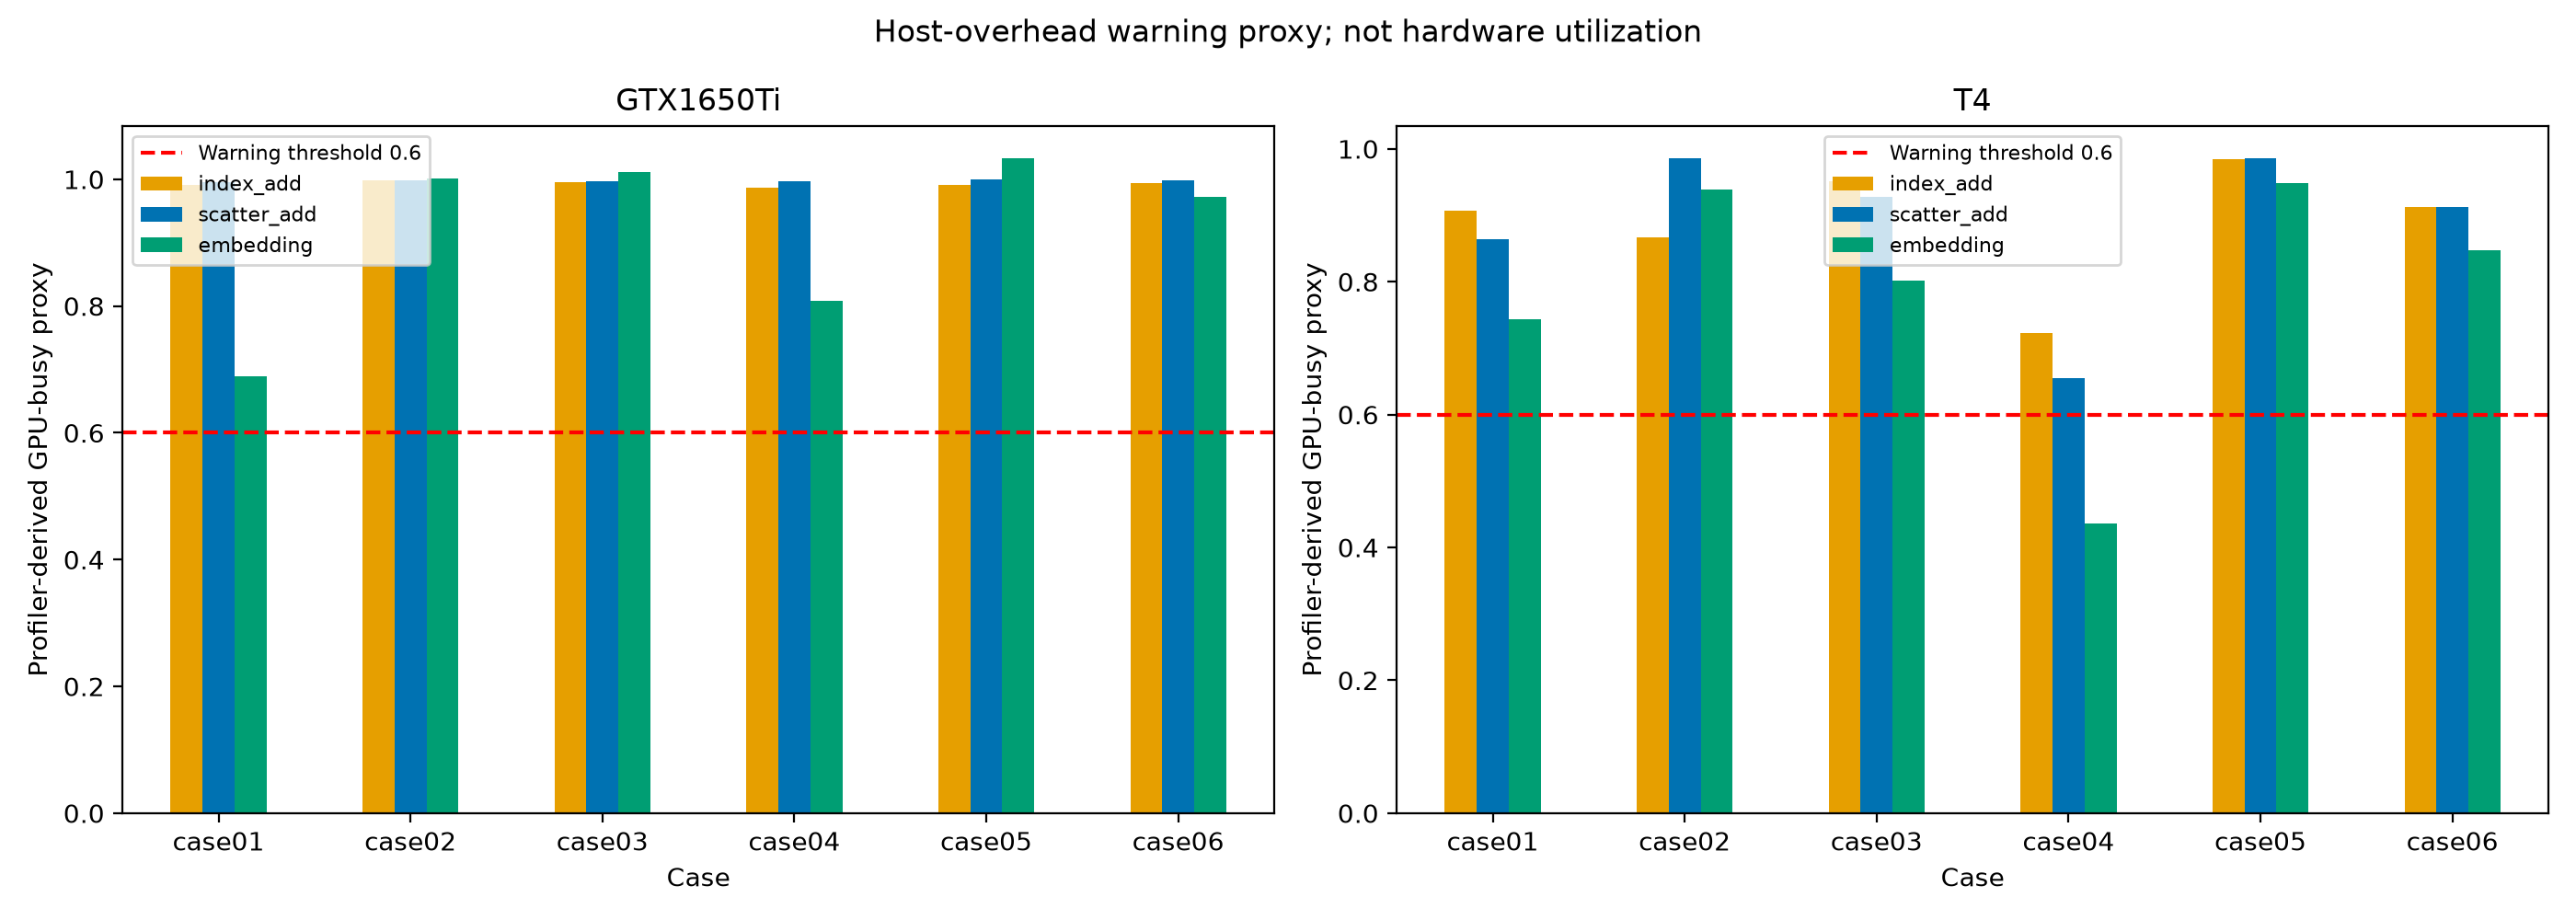
\includegraphics[width=0.95\linewidth]{figures/phase3_gpu_busy_fraction_by_case_operation.png}
\caption{Profiler-derived GPU-busy proxy by representative case and operation. The proxy is diagnostic only and is not interpreted as hardware utilization.}
\label{fig:phase3-gpu-busy}
\end{figure*}

The kernel-category summary in Table~\ref{tab:phase3-kernel-category-summary} and Figure~\ref{fig:phase3-kernel-category-share} shows that the three API paths are not merely different syntactic forms of the same CUDA behavior. The \texttt{index\_\allowbreak add} path is dominated by indexed accumulation kernels, the \texttt{scatter\_\allowbreak add} path is dominated by scatter/gather-style accumulation kernels, and the embedding backward path uses a multi-kernel composition that includes accumulation as well as sorting, scanning, or uniqueness-related components.

% Source summary: sparse-gradient/phase3_comparison_v2/phase3_kernel_category_summary.csv.
% Detailed per-case rows can be moved to an appendix or supplementary material later.
\begin{table*}[t]
\centering
\fontsize{9}{11}\selectfont
\caption{Mean CUDA kernel-category shares for the representative Phase 3 profiles. Shares are averaged across the profiled cases for each environment and operation.}
\label{tab:phase3-kernel-category-summary}
\setlength{\tabcolsep}{3pt}
\renewcommand{\arraystretch}{1.12}
\begin{tabularx}{\linewidth}{@{}l l >{\raggedright\arraybackslash}X >{\raggedleft\arraybackslash}p{1.5cm} >{\raggedright\arraybackslash}X >{\raggedleft\arraybackslash}p{1.6cm} >{\raggedleft\arraybackslash}p{1.0cm}@{}}
\toprule
Environment & Operation & Dominant category & Dominant share & Secondary category & Secondary share & Other share \\
\midrule
GTX1650Ti & embedding & \texttt{embedding\_\allowbreak accumulate} & 0.8271 & \texttt{sort\_\allowbreak scan\_\allowbreak unique} & 0.1217 & -- \\
GTX1650Ti & \texttt{index\_add} & \texttt{index\_\allowbreak add\_\allowbreak accumulate} & 0.9677 & \texttt{zero\_\allowbreak fill\_\allowbreak memset} & 0.0323 & -- \\
GTX1650Ti & \texttt{scatter\_add} & \texttt{scatter\_\allowbreak add\_\allowbreak accumulate} & 0.9817 & \texttt{zero\_\allowbreak fill\_\allowbreak memset} & 0.0183 & -- \\
T4 & embedding & \texttt{embedding\_\allowbreak accumulate} & 0.6697 & \texttt{sort\_\allowbreak scan\_\allowbreak unique} & 0.2342 & 0.0347 \\
T4 & \texttt{index\_add} & \texttt{index\_\allowbreak add\_\allowbreak accumulate} & 0.9647 & \texttt{zero\_\allowbreak fill\_\allowbreak memset} & 0.0353 & -- \\
T4 & \texttt{scatter\_add} & \texttt{scatter\_\allowbreak add\_\allowbreak accumulate} & 0.9518 & \texttt{zero\_\allowbreak fill\_\allowbreak memset} & 0.0482 & -- \\
\bottomrule
\end{tabularx}
\end{table*}


\begin{figure*}[t]
\centering
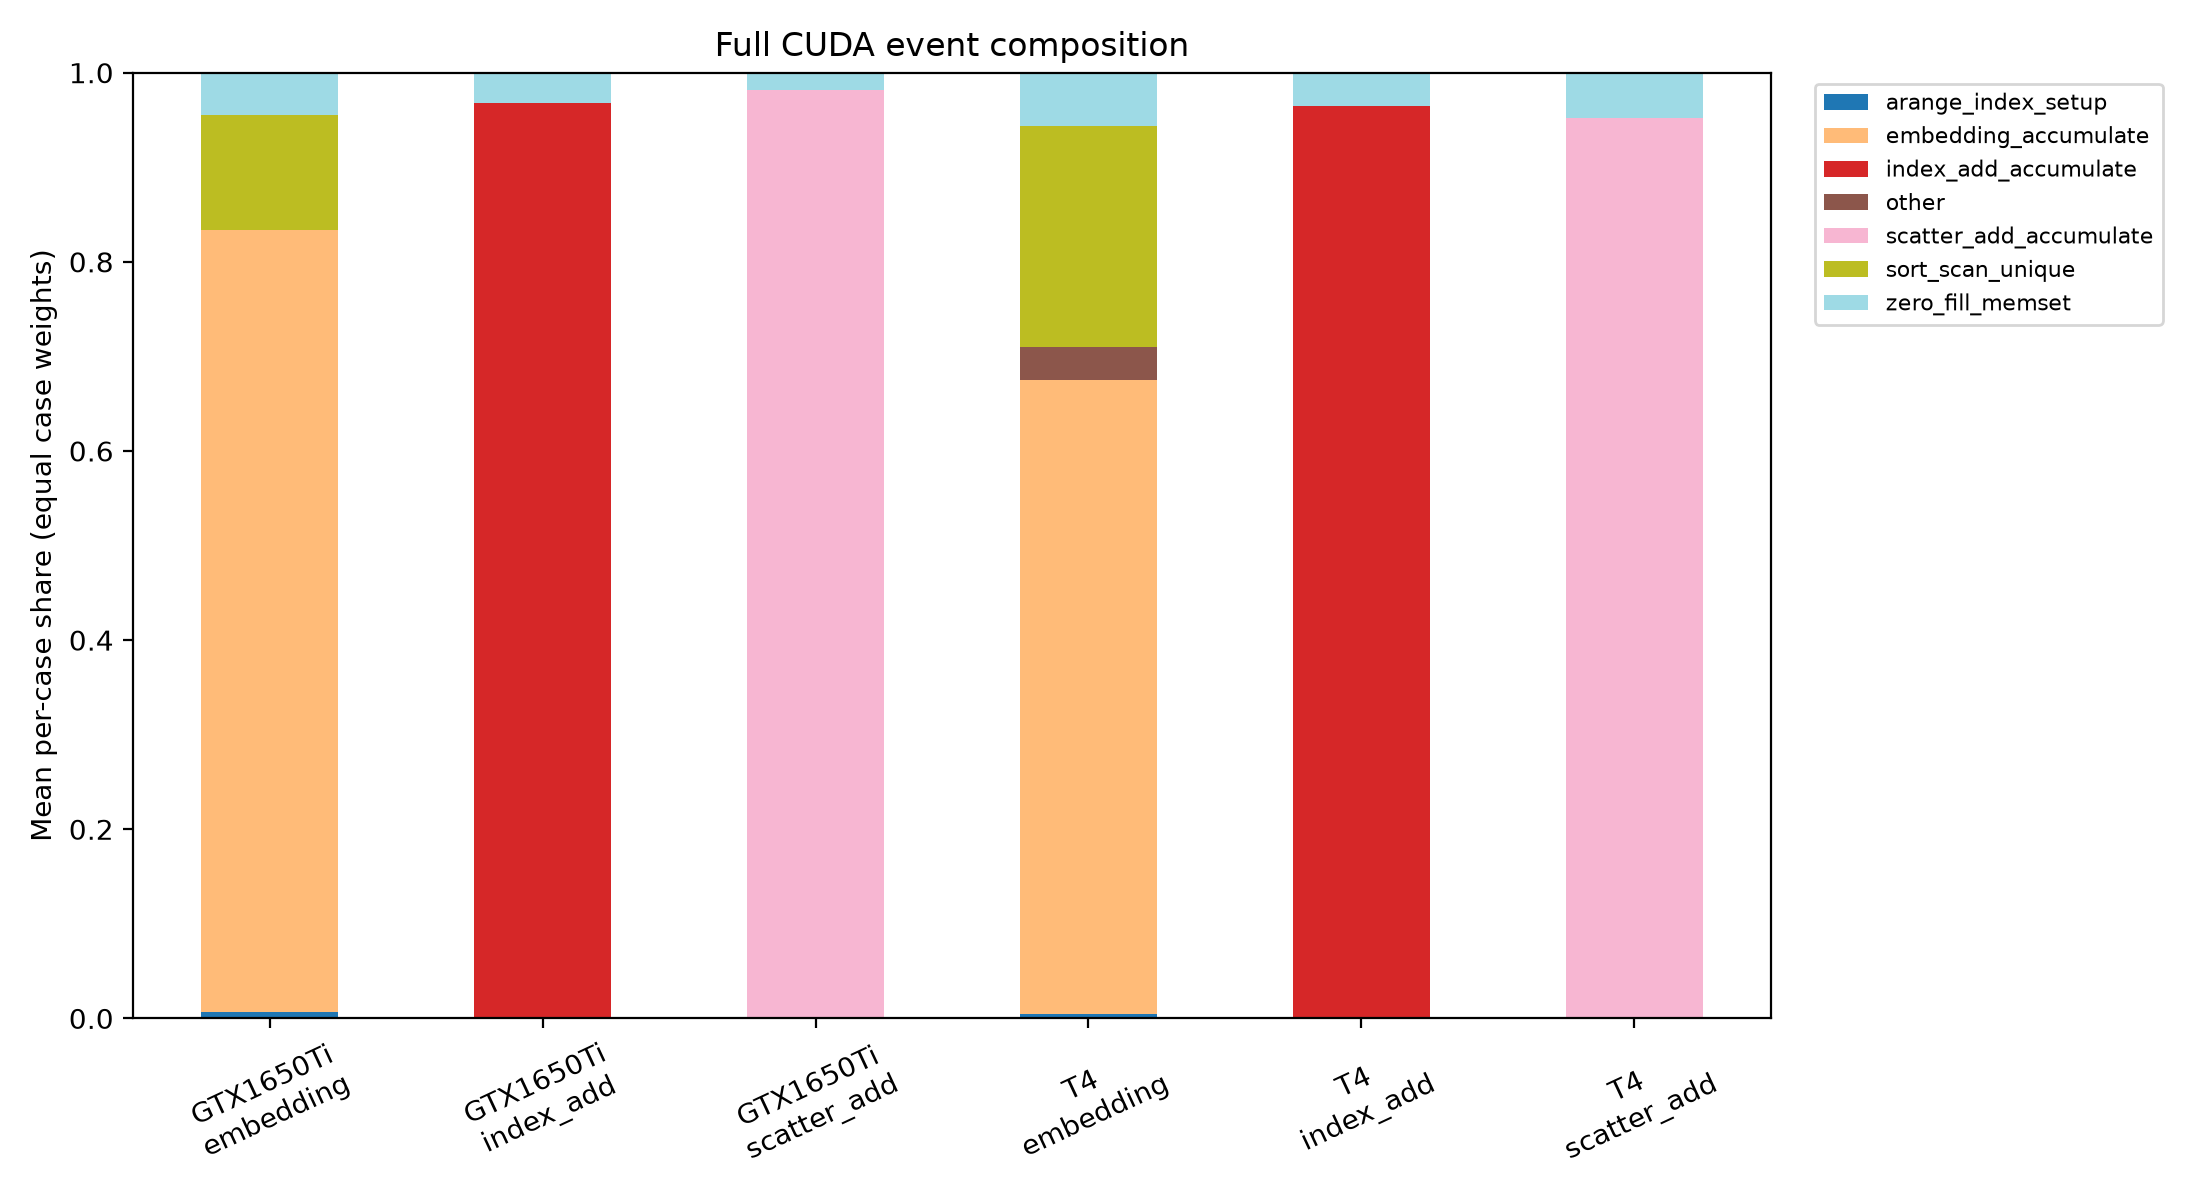
\includegraphics[width=0.95\linewidth]{figures/phase3_kernel_category_share.png}
\caption{Mean CUDA kernel-category share for the representative Phase 3 profiles. Category shares are computed from CUDA device events and summarize observed execution-path composition.}
\label{fig:phase3-kernel-category-share}
\end{figure*}

The mean category shares support the intended execution-path interpretation. In both environments, \texttt{index\_\allowbreak add} is dominated by the \texttt{index\_\allowbreak add\_\allowbreak accumulate} category, while \texttt{scatter\_\allowbreak add} is dominated by the \texttt{scatter\_\allowbreak add\_\allowbreak accumulate} category. The embedding backward path is dominated by \texttt{embedding\_\allowbreak accumulate}, but it also contains a non-trivial \texttt{sort\_\allowbreak scan\_\allowbreak unique} component. The \texttt{other} category remains below the selected control threshold, which reduces the risk that the main attribution is hiding a large unclassified portion of CUDA time.

\subsection{Case-Level Cross-Environment Comparison}

The Phase 3 case-level comparison links the representative profiling subset to both environments and to the broader Phase 2 grid. Table~\ref{tab:phase3-case-comparison} summarizes the raw case-level winners, margins, and winner-relation categories for the six representative cases.

% Source: ../sparse-gradient/phase3_comparison_v2/phase3_case_comparison.csv
\begin{table*}[t]
\centering
\fontsize{9}{11}\selectfont
\caption{Phase 3 case-level comparison across environments.}
\label{tab:phase3-case-comparison}
\setlength{\tabcolsep}{3pt}
\renewcommand{\arraystretch}{1.12}
\begin{tabular*}{\textwidth}{@{\extracolsep{\fill}}lrrrrl@{}}
\toprule
Case & Local winner & T4 winner & \shortstack{Local\\margin} & \shortstack{T4\\margin} & \shortstack{Winner\\relation} \\
\midrule
case01 & index\_add & scatter\_add & 1.670 & 1.022 & reversal near-tie \\
case02 & embedding & embedding & 2.631 & 1.706 & same decisive \\
case03 & embedding & scatter\_add & 1.116 & 1.186 & reversal decisive \\
case04 & index\_add & index\_add & 1.197 & 1.058 & same decisive \\
case05 & embedding & scatter\_add & 1.257 & 1.285 & reversal decisive \\
case06 & embedding & scatter\_add & 1.015 & 1.040 & reversal near-tie \\
\bottomrule
\end{tabular*}
\end{table*}

Two cases provide the strongest evidence of a cross-environment reversal. In case03, the GTX1650Ti stack selects \texttt{embedding} decisively, while the T4 stack selects \texttt{scatter\_\allowbreak add} decisively. In case05, the same pattern appears again: the GTX1650Ti stack selects \texttt{embedding}, whereas the T4 stack selects \texttt{scatter\_\allowbreak add}. Both cases pass the stronger clean-reversal gates in the comparison analysis: they are decisively separated, have clean GPU-busy proxy status, and use exact index pairing across environments.

Figure~\ref{fig:phase3-case-winner-comparison} visualizes the case-level winner comparison. The figure shows a mixture of agreement, near-ties, and decisive reversals within the diagnostic subset.

\begin{figure*}[t]
\centering
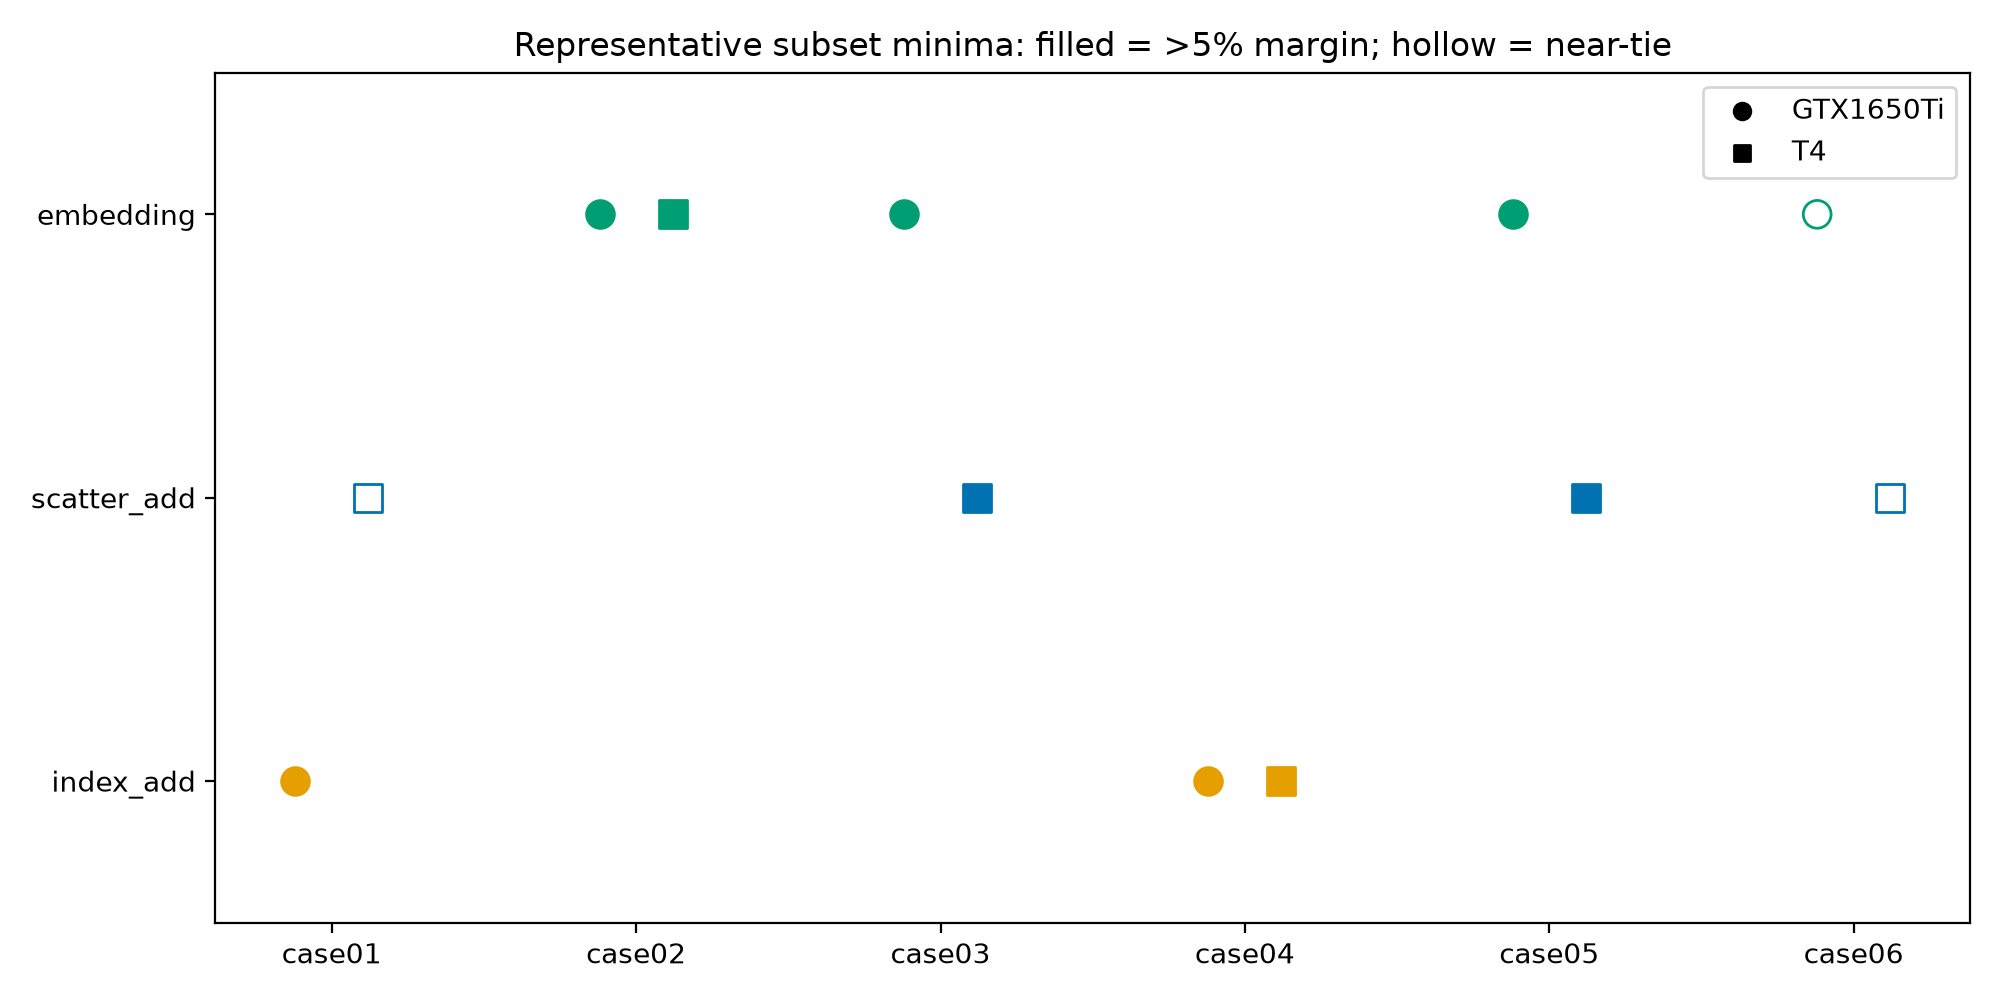
\includegraphics[width=0.95\linewidth]{figures/phase3_case_winner_comparison.png}
\caption{Representative Phase 3 winner comparison across environments. Filled markers indicate decisive practical-margin winners, while near-ties are interpreted as weak evidence.}
\label{fig:phase3-case-winner-comparison}
\end{figure*}

The remaining cases serve as controls or cautionary examples rather than strong claims of representativeness. In case02, both environments select \texttt{embedding} decisively. In case04, both environments select \texttt{index\_\allowbreak add} decisively, although the T4 \texttt{embedding} row has a host-overhead warning and therefore prevents a fully GPU-clean claim for that case. Cases case01 and case06 exhibit different raw winners across environments, but at least one side is a near-tie, so these cases are treated as weak evidence rather than decisive reversals.

The profiled cases were linked back to the broader Phase~2 grid. The strongest support comes from case03 and case05, where both the grid and profiling agree on a decisive reversal: the GTX1650Ti stack favors \texttt{Embedding.\allowbreak backward}, whereas the T4 stack favors \texttt{scatter\_\allowbreak add}. The remaining cases serve as controls or cautionary examples involving agreement, near-ties, or host-overhead warnings; the subset is diagnostic rather than statistically representative of the full grid.

The case-level evidence therefore reinforces the grid-level result without replacing it. Phase 2 establishes the broader matched-performance pattern, while Phase 3 explains selected cases in terms of execution-path differences. The combination of the two phases is stronger than either alone: the timing grid shows that the fastest API changes across environments, and the profiler shows that the compared APIs exercise distinct CUDA paths.

\subsection{CUDA Path Attribution}

Execution-path conclusions require consistent kernel-category attribution. Cross-environment reversal claims additionally require practical-margin separation, stable timing, exact index pairing, and no host-overhead warning.

% Evidence criteria retained in prose; diagnostic table excluded from the main flow.
% % Source: ../sparse-gradient/phase3_comparison_v2/phase3_claim_checks.csv
\begin{table}[tbp]
\centering
\fontsize{9}{11}\selectfont
\caption{Phase 3 claim-check status and source cautions.}
\label{tab:phase3-claim-checks}
\resizebox{\linewidth}{!}{%
\begin{tabular}{lp{0.12\linewidth}p{0.30\linewidth}p{0.36\linewidth}}
\toprule
Check & Passed & Supporting numbers & Caution \\
\midrule
index\_add\_path\_dominance & True & GTX1650Ti=0.9677; T4=0.9647 & Full-event CUDA category shares required. \\
scatter\_add\_path\_dominance & True & GTX1650Ti=0.9817; T4=0.9518 & Full-event CUDA category shares required. \\
embedding\_accumulation\_present & True & GTX1650Ti=0.8271; T4=0.6697 & Full-event CUDA category shares required. \\
embedding\_sort\_scan\_present & True & GTX1650Ti=0.1217; T4=0.2342 & Full-event CUDA category shares required. \\
other\_share\_controlled & True & T4/embedding=0.03467 & Unknown kernels substantial at mean other share $\geq 0.2$. \\
phase2\_environment\_difference\_present & True & GTX1650Ti=embedding; T4=scatter\_add; T4\_repeat=scatter\_add & Expected most-frequent decisive API required in the local run and both T4 runs. \\
representative\_reversals\_present & True & case03, case05 & Representative subset is illustrative, not statistical. \\
\bottomrule
\end{tabular}
}%
\end{table}

The \texttt{index\_\allowbreak add} path is dominated by the \texttt{index\_\allowbreak add\_\allowbreak accumulate} category in both environments, and the \texttt{scatter\_\allowbreak add} path is dominated by the \texttt{scatter\_\allowbreak add\_\allowbreak accumulate} category in both environments. This supports the claim that the two APIs dispatch to distinct CUDA reduction paths under the profiled workloads.

The embedding backward path contains a dominant accumulation component, but it also includes sorting, scanning, or uniqueness-related work. This distinguishes \texttt{Embedding.\allowbreak backward} from the direct \texttt{index\_\allowbreak add} and \texttt{scatter\_\allowbreak add} paths. The result is consistent with the interpretation that embedding backward is a specialized framework path rather than a simple alias for either direct accumulation API.

Within the profiled subset, case03 and case05 satisfy the strict evidence conditions: they are decisive reversals, they are not host-warning cases, they have stable timing evidence, and they use exact index pairing. These cases therefore support the paper-level statement that the relative cost of sparse-index accumulation paths can change with workload and software/hardware stack.

At the same time, the attribution remains conservative. The kernel categories are based on profiler event names and CUDA event durations, not on low-level hardware counters. They support execution-path attribution within the measured stacks; the hardware-causality limitations are detailed in Section~\ref{sec:methodology}.

% Standalone staged subsection; not inserted into the existing manuscript.
\subsection{Training-step proxy}
\label{sec:phase4-training-proxy}

To examine whether the sparse-index accumulation effects observed in isolated
measurements persist in a broader backpropagation-style setting, we introduced a
small synthetic training-step proxy. The proxy combines indexed lookup, grouped
mean pooling, a scalar linear prediction head, mean-squared error, and backward
propagation. The three variants use identical inputs, pooling, head, and loss.
The \texttt{embedding\_\allowbreak backward\_\allowbreak proxy} variant uses native dense Embedding
backward, whereas \texttt{index\_\allowbreak add\_\allowbreak proxy} and
\texttt{scatter\_\allowbreak add\_\allowbreak proxy} use custom autograd lookup nodes that allocate a
dense zero gradient and accumulate row gradients with the corresponding PyTorch
API.

Two timing scopes were recorded. The \texttt{proxy\_\allowbreak step} scope measures the
complete synthetic step: lookup, pooling, prediction, loss, and gradients for the
table, head, and bias. The \texttt{accumulation\_\allowbreak region} scope separately replays
backward through a retained lookup graph with fixed upstream gradients. This
second scope is diagnostic only: it includes autograd dispatch, dense gradient
allocation and zeroing, and accumulation, but it is not an exact decomposition of
the proxy step and must not be subtracted from total-step latency.

Each environment was evaluated with five seeds and 24 configurations per seed,
giving 120 seed--configuration observations per environment. The grid varied the
number of rows, number of references, embedding dimension, and index
distribution. All included runs completed successfully, and all configurations
and variants passed the recorded validation checks. As in the preceding
experiments, a variant is counted as a winner only when the runner-up median is
strictly more than 5\% slower; otherwise the observation is classified as a
practical tie.

Table~\ref{tab:phase4-winner-counts} and
Figure~\ref{fig:phase4-winner-counts} summarize the results. On the GTX1650Ti stack, \texttt{index\_\allowbreak add} dominated both scopes, winning 83 of 120
proxy-step observations and 98 of 120 accumulation-region observations. Native
Embedding won 10 observations in each scope, while the remaining cases were
classified as practical ties. On the T4 stack, practical ties dominated: 95 of
120 proxy-step observations and 78 of 120 accumulation-region observations. Among
the resolved T4 cases, the proxy step favored \texttt{scatter\_\allowbreak add} in 25
observations, while the accumulation-region diagnostic favored
\texttt{scatter\_\allowbreak add} in 39 observations and \texttt{index\_\allowbreak add} in three.

\begin{table*}[t]
\centering\fontsize{9}{11}\selectfont
\caption{Phase~4 winners under the strictly greater than 5\% practical-margin rule. Each environment contributes 120 seed--configuration observations. Region replay denotes the separate accumulation diagnostic scope.}
\label{tab:phase4-winner-counts}
\setlength{\tabcolsep}{3pt}
\renewcommand{\arraystretch}{1.12}
\begin{tabular*}{\textwidth}{@{\extracolsep{\fill}}llrrrrr@{}}
\toprule
Environment & Scope & \texttt{index\_add} & \texttt{scatter\_add} & Embedding & Tie & Total \\
\midrule
GTX1650Ti & Proxy step & 83 & 0 & 10 & 27 & 120 \\
GTX1650Ti & Region replay & 98 & 0 & 10 & 12 & 120 \\
T4 & Proxy step & 0 & 25 & 0 & 95 & 120 \\
T4 & Region replay & 3 & 39 & 0 & 78 & 120 \\
\bottomrule
\end{tabular*}
\end{table*}
% \begin{table}[tbp]
\centering\fontsize{9}{11}\selectfont
\caption{Descriptive Phase~4 outcomes by environment. The contrast is not attributed to GPU hardware alone because the software and host environments also differ.}
\label{tab:phase4-environment-comparison}
\setlength{\tabcolsep}{3pt}
\begin{tabularx}{\linewidth}{lXXX}
\toprule
Environment & Proxy-step outcome & Region-replay outcome & Interpretation \\
\midrule
GTX1650Ti & \texttt{index\_add}: 83/120 & \texttt{index\_add}: 98/120 & The local stack most often favors the custom \texttt{index\_add} path. \\
T4 & Tie: 95/120 & Tie: 78/120 & Most observations are unresolved; resolved cases mainly favor \texttt{scatter\_add}. \\
\bottomrule
\end{tabularx}
\end{table}

\begin{figure*}[t]
\centering
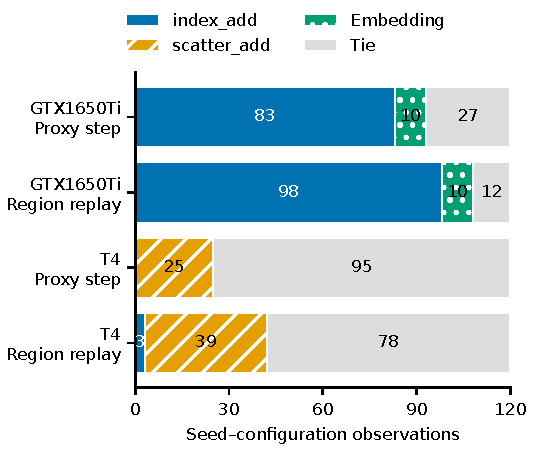
\includegraphics[width=0.60\linewidth]{figures/phase4_winner_counts_by_environment.pdf}
\caption{Phase~4 practical-margin winner counts across five seeds and 24
configurations per environment. Region replay denotes the separate accumulation
diagnostic scope. Ties are retained explicitly.}
\label{fig:phase4-winner-counts}
\end{figure*}

The proxy results reinforce the central conclusion that sparse-index accumulation
performance is conditional rather than universal. In the GTX1650Ti stack, the custom \texttt{index\_\allowbreak add} backward path was most often favored.
In the T4 stack, most observations were unresolved by the 5\% practical
margin rule, and the resolved cases mainly favored \texttt{scatter\_\allowbreak add}. This
contrast should not be interpreted as isolated GPU causality, because the two
environments also differ in PyTorch version, CUDA version, operating system, and
host settings. Instead, the result shows that rankings obtained from isolated
sparse-index accumulation measurements should not be transferred mechanically to
a training-step-like context without measurement.

This proxy remains deliberately limited. It does not measure convergence,
optimizer state, data loading, distributed training, or production-scale model
throughput. The manual variants use custom autograd lookup nodes, so the
comparison is at the API/path level and includes dispatch and graph overhead
rather than pure kernel speed. The \texttt{accumulation\_\allowbreak region} scope is a
diagnostic replay, not a decomposition of the proxy step.

\subsection{Practical-Margin Threshold Sensitivity}
\label{sec:threshold-sensitivity}

The primary analysis uses a strictly greater than 5\% practical-margin rule to avoid treating small median-latency differences as decisive API wins. To check whether the qualitative conclusions depend on this specific threshold, we recomputed winner counts using 2\%, 5\%, and 10\% thresholds from the saved per-variant median-latency artifacts. The fastest path is counted as a winner only when the runner-up median divided by the fastest median, minus one, exceeds the selected threshold. These sensitivity checks are descriptive robustness checks, not statistical tests; the main analysis retains the 5\% rule.

Table~\ref{tab:threshold-sensitivity-phase2} shows the Phase~2 sensitivity results over the same 162 matched configuration--draw observations per run. The recomputed 5\% counts reproduce the main analysis. Tie counts change by design: lower thresholds reduce their number, while higher thresholds increase it. The qualitative Phase~2 pattern remains across the tested thresholds: the GTX1650Ti stack most often favors \texttt{Embedding.\allowbreak backward}, while the T4 stack and its repeat run most often favor \texttt{scatter\_\allowbreak add}.

\begin{table*}[t]
\centering\fontsize{9}{11}\selectfont
\caption{Threshold sensitivity of Phase~2 winner counts. The main paper uses the strictly greater than 5\% practical-margin rule; 2\% and 10\% are reported only as sensitivity checks.}
\label{tab:threshold-sensitivity-phase2}
\setlength{\tabcolsep}{3pt}
\renewcommand{\arraystretch}{1.12}
\begin{tabular*}{\textwidth}{@{\extracolsep{\fill}}llrrrrr@{}}
\toprule
Environment & Threshold & \texttt{index\_add} & \texttt{scatter\_add} & Embedding & Tie & Total \\
\midrule
GTX1650Ti & 2\% & 61 & 0 & 99 & 2 & 162 \\
GTX1650Ti & 5\% & 60 & 0 & 96 & 6 & 162 \\
GTX1650Ti & 10\% & 52 & 0 & 91 & 19 & 162 \\
T4 & 2\% & 9 & 113 & 28 & 12 & 162 \\
T4 & 5\% & 5 & 92 & 25 & 40 & 162 \\
T4 & 10\% & 3 & 78 & 21 & 60 & 162 \\
T4 repeat & 2\% & 4 & 120 & 30 & 8 & 162 \\
T4 repeat & 5\% & 1 & 93 & 27 & 41 & 162 \\
T4 repeat & 10\% & 0 & 81 & 22 & 59 & 162 \\
\bottomrule
\end{tabular*}
\end{table*}


Table~\ref{tab:threshold-sensitivity-phase4} shows the corresponding Phase~4 sensitivity results for 120 seed--configuration observations per environment and scope. Its 5\% counts also reproduce the main analysis. On the GTX1650Ti stack, \texttt{index\_\allowbreak add} remains the most frequent resolved winner in both scopes across the tested thresholds. However, the proxy-step result becomes nearly balanced with ties at 10\% (58 \texttt{index\_\allowbreak add} wins versus 57 ties), while the accumulation replay remains more stable with 97 \texttt{index\_\allowbreak add} wins at the same threshold.

The T4 proxy step remains majority-tied at all three thresholds, with resolved cases mainly favoring \texttt{scatter\_\allowbreak add}. In the T4 accumulation replay, ties rise from 40/120 at 2\% to 78/120 at 5\% and 99/120 at 10\%; at 2\%, \texttt{scatter\_\allowbreak add} is the largest category with 58 wins. These results show that the qualitative workload-, scope-, and stack-dependent interpretation is stable, while the absolute balance between resolved outcomes and ties is threshold-sensitive.

\begin{table*}[t]
\centering\fontsize{9}{11}\selectfont
\caption{Threshold sensitivity of Phase~4 proxy winner counts. The main paper uses the strictly greater than 5\% practical-margin rule; 2\% and 10\% are reported only as sensitivity checks.}
\label{tab:threshold-sensitivity-phase4}
\setlength{\tabcolsep}{3pt}
\renewcommand{\arraystretch}{1.12}
\begin{tabular*}{\textwidth}{@{\extracolsep{\fill}}lllrrrrr@{}}
\toprule
Environment & Scope & Threshold & \texttt{index\_add} & \texttt{scatter\_add} & Embedding & Tie & Total \\
\midrule
GTX1650Ti & Proxy step & 2\% & 96 & 1 & 11 & 12 & 120 \\
GTX1650Ti & Proxy step & 5\% & 83 & 0 & 10 & 27 & 120 \\
GTX1650Ti & Proxy step & 10\% & 58 & 0 & 5 & 57 & 120 \\
GTX1650Ti & Region replay & 2\% & 106 & 0 & 11 & 3 & 120 \\
GTX1650Ti & Region replay & 5\% & 98 & 0 & 10 & 12 & 120 \\
GTX1650Ti & Region replay & 10\% & 97 & 0 & 10 & 13 & 120 \\
T4 & Proxy step & 2\% & 2 & 42 & 0 & 76 & 120 \\
T4 & Proxy step & 5\% & 0 & 25 & 0 & 95 & 120 \\
T4 & Proxy step & 10\% & 0 & 18 & 0 & 102 & 120 \\
T4 & Region replay & 2\% & 22 & 58 & 0 & 40 & 120 \\
T4 & Region replay & 5\% & 3 & 39 & 0 & 78 & 120 \\
T4 & Region replay & 10\% & 0 & 21 & 0 & 99 & 120 \\
\bottomrule
\end{tabular*}
\end{table*}


As an additional descriptive stability check, we computed bootstrap intervals for selected aggregate winner shares from the saved 5\% winner classifications. These intervals are not hypothesis tests and do not support inference to all possible workloads, GPUs, or software versions. They summarize resampling variability conditional on the saved observations.

In Phase~2, the dominant-share intervals preserve the same qualitative pattern. The GTX1650Ti \texttt{Embedding.\allowbreak backward} share is 59.3\%, with a 95\% descriptive interval of 51.9--66.7\%. The \texttt{scatter\_\allowbreak add} shares are 56.8\% on T4 and 57.4\% on the T4 repeat, with intervals of 49.4--64.2\% and 50.0--64.8\%, respectively. In Phase~4, observation-level intervals support the GTX1650Ti \texttt{index\_\allowbreak add} tendency and the T4 tie-heavy interpretation, while configuration-cluster intervals are wider. For example, the GTX1650Ti proxy-step \texttt{index\_\allowbreak add} share is 69.2\%, with an observation-level interval of 60.8--77.5\% and a configuration-cluster interval of 50.8--85.8\%. The wider cluster interval reinforces that the proxy should be interpreted as a controlled descriptive study rather than a population-level statistical estimate.

\subsection{Result-Level Discussion}

The combined results answer the central question of the study: standard PyTorch CUDA APIs that express related sparse-index accumulation behavior do not necessarily have interchangeable performance characteristics during backpropagation-style workloads. In the matched Phase 2 grid, the GTX1650Ti stack most often favors the embedding backward path, whereas the T4 stack and its repeat run most often favor \texttt{scatter\_\allowbreak add}. In the representative Phase 3 profiles, the strongest reversal cases show the same pattern at the case level: GTX1650Ti execution favors \texttt{embedding}, while T4 execution favors \texttt{scatter\_\allowbreak add}.

The results also show why the difference should not be reduced to a simple API ranking. Some representative cases agree across environments, some differ only as near-ties, and two cases provide strong decisive reversals. This mixed behavior indicates that the best operation depends on workload shape, index distribution, duplicate structure, and the software/hardware stack. A recommendation such as ``always use \texttt{scatter\_\allowbreak add}'' or ``always use \texttt{Embedding.\allowbreak backward}'' would not be supported by the evidence.

The execution-path attribution provides a practical explanation for this behavior. Although the operations represent related accumulation-style computations, they dispatch to different CUDA paths. \texttt{index\_\allowbreak add} and \texttt{scatter\_\allowbreak add} use different direct accumulation kernels, while \texttt{Embedding.\allowbreak backward} uses a multi-kernel path that includes embedding-specific accumulation and sorting or segmentation-related work. These differences create opportunities for the relative cost of the APIs to change when the workload or execution stack changes.

For practitioners, the results suggest that sparse-gradient accumulation paths in AI training should not be selected purely from high-level API semantics. When sparse-index accumulation is a relevant part of the backward pass, especially in embedding-heavy models, recommender workloads, or other skewed-index settings, the actual execution path and target environment can materially affect performance. Microbenchmarking and profiler inspection remain useful tools for identifying which API path is most appropriate for a specific workload and deployment stack.

Finally, the results define the boundary of the present evidence. The study characterizes controlled sparse-index accumulation workloads and representative profiler cases; it does not measure full model training throughput, convergence behavior, distributed execution, or custom CUDA alternatives. Therefore, the contribution is best understood as a controlled characterization of PyTorch CUDA sparse-index gradient accumulation paths during backpropagation-style computation, rather than as a complete benchmark of AI training systems.
\section{General Discussion}
\label{sec:general-discussion}

\subsection{Significance for AI Training Workloads}

Sparse-index accumulation matters in embedding-heavy and sparse-feature training, where repeated references route many source vectors into a dense gradient structure \citep{mudigere2022neo,liu2024embark}. Its cost can depend on workload shape, duplication, skew, and framework dispatch even when dense linear algebra dominates other parts of a model.

The contribution is a reproducible performance characterization and measurement-backed interpretation of these paths. High-level API similarity does not imply CUDA execution-path similarity: profiler summaries expose distinct kernel compositions, and the isolated and proxy results show workload-, scope-, and stack-dependent behavior. The winner-map and regret analyses turn these observations into descriptive guidance, culminating in a tie-aware selection protocol for the target workload and execution stack.

\subsection{Practical Implications}

The most direct practical implication is that sparse-gradient accumulation paths should be benchmarked under the intended workload and execution stack. The fastest path depends on the workload shape, duplicate-index structure, feature dimension, and software/hardware stack.

Exploratory grouped summaries add practical but non-predictive rule-of-thumb context to these measurements. They identify workload-feature combinations associated with recurring API preferences or tie-heavy outcomes in the saved grid. These descriptive patterns should be validated on the target workload and stack before informing implementation choices.

\begin{figure*}[t]
\centering
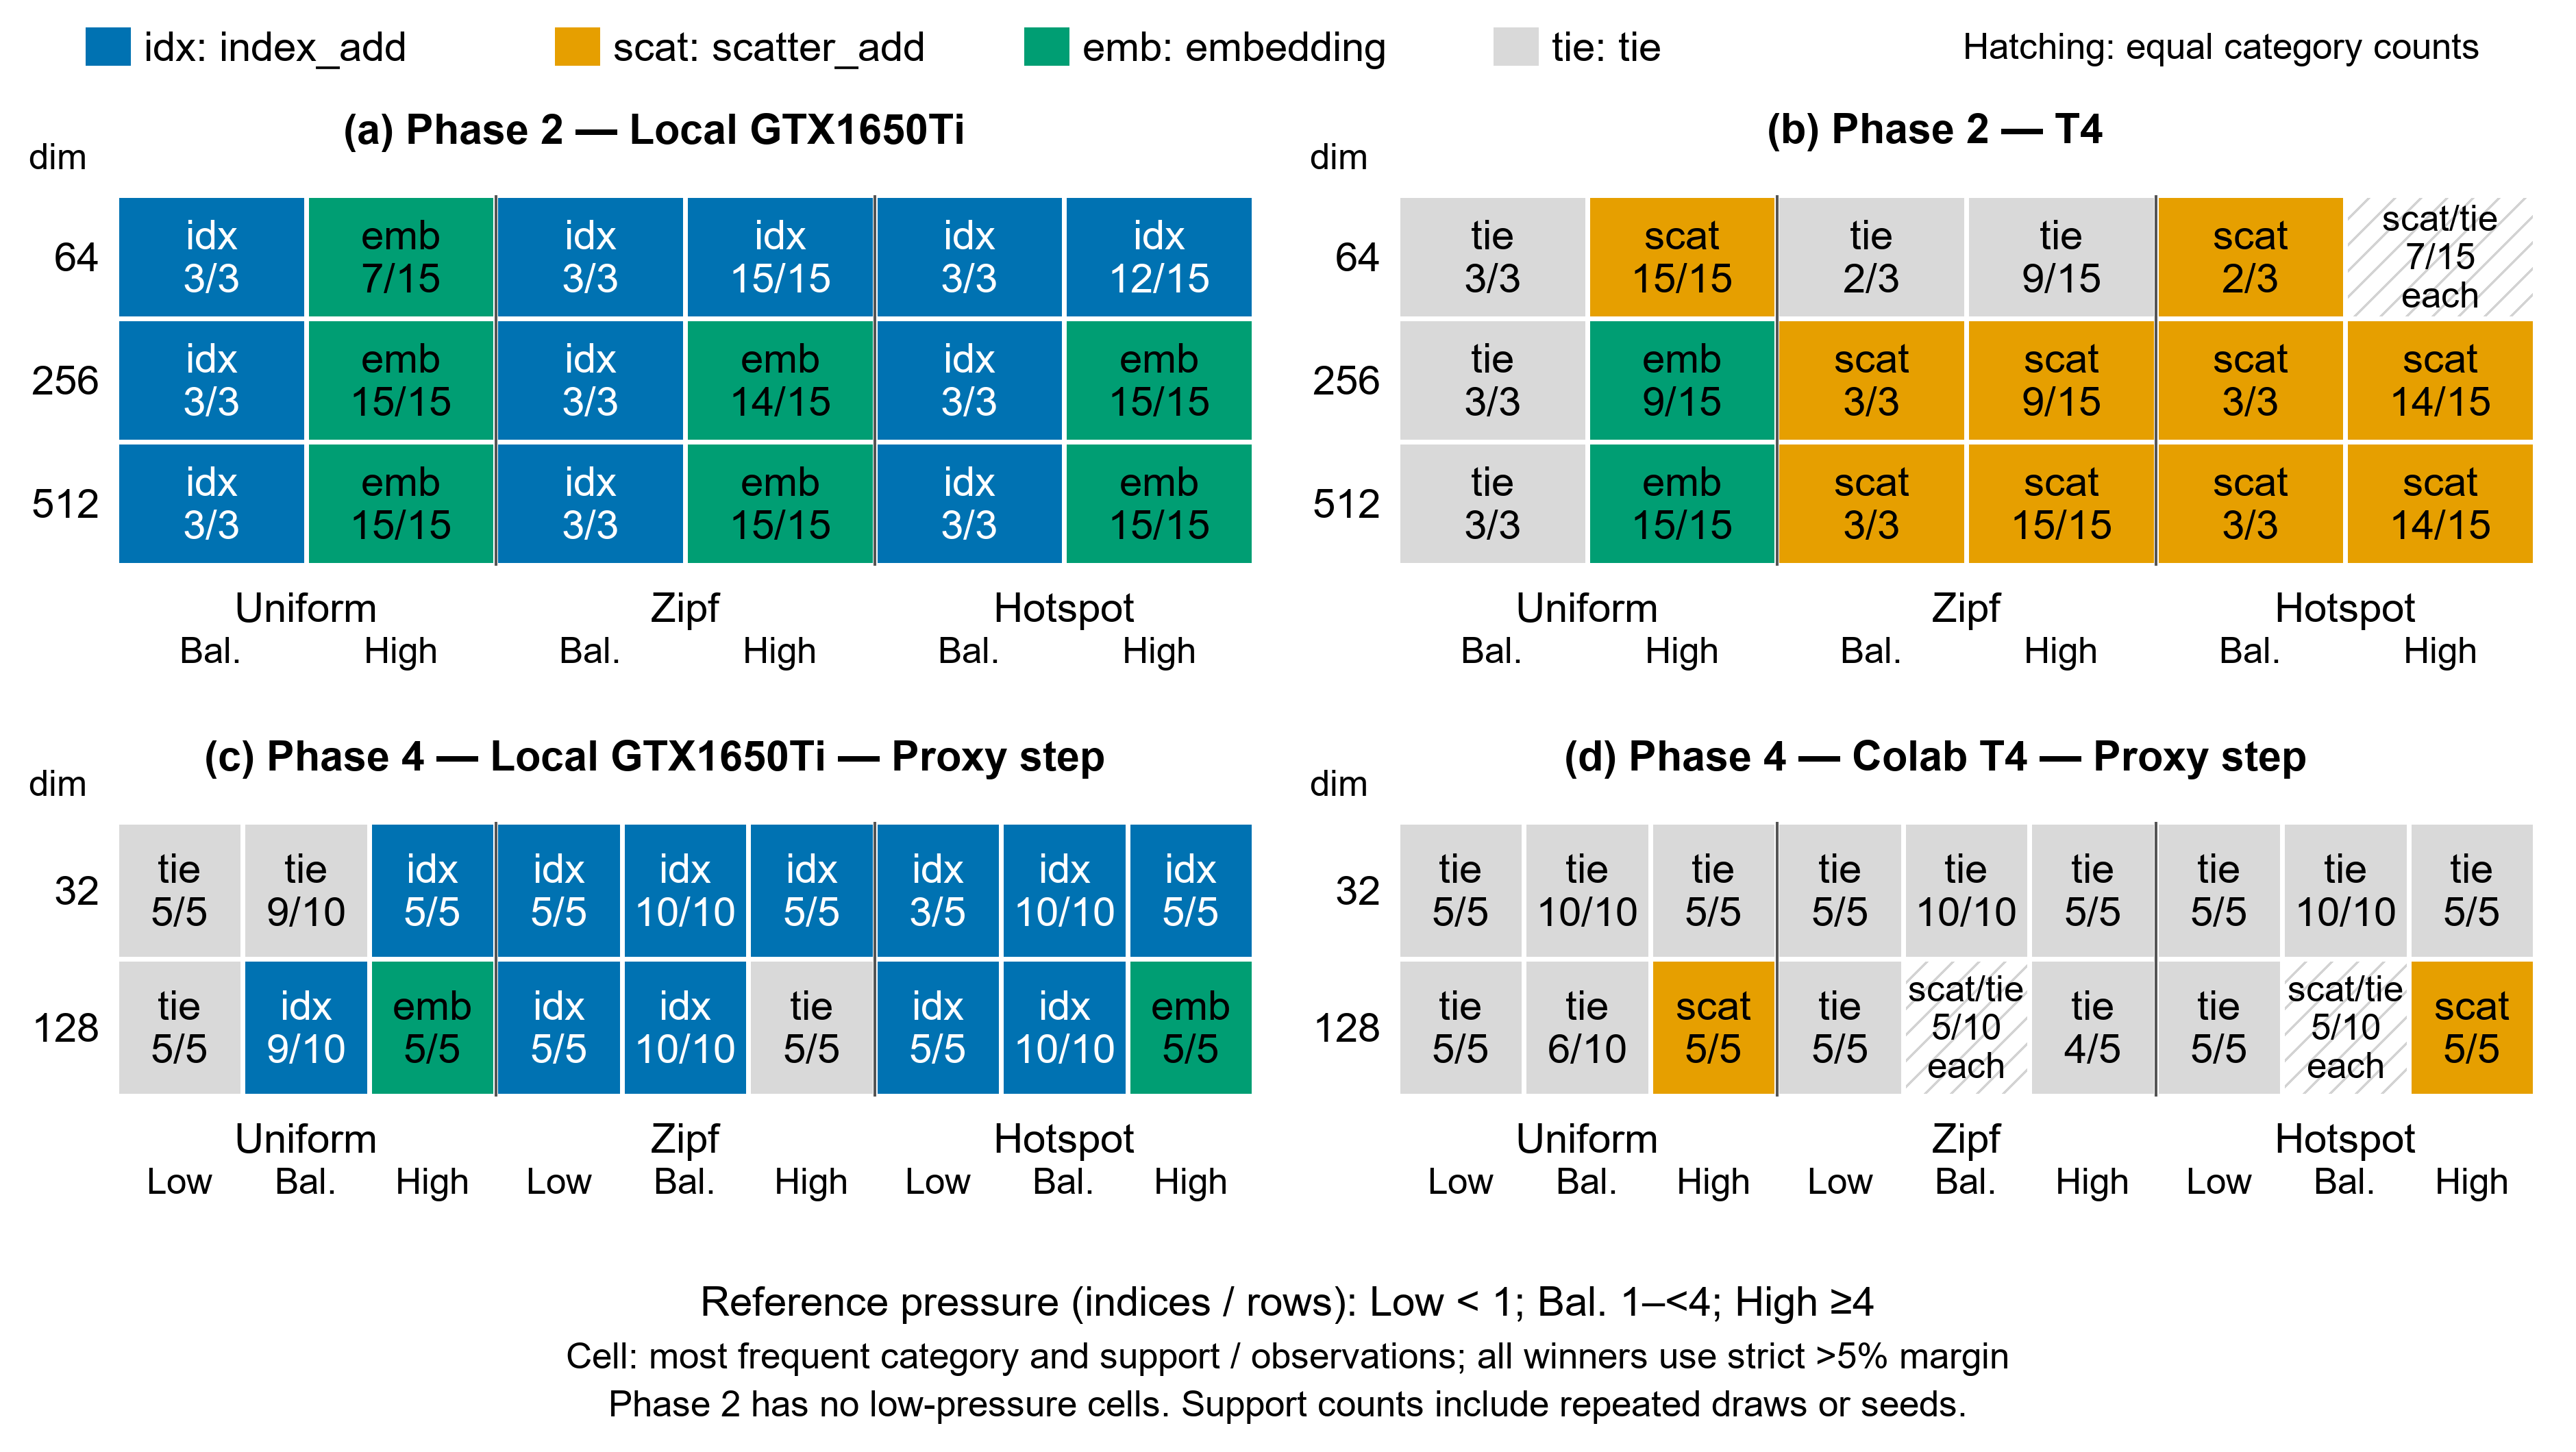
\includegraphics[width=\linewidth]{figures/winner_maps_four_panel.png}
\caption{Descriptive winner maps for selected Phase~2 and Phase~4 analyses under the strict greater-than 5\% practical-margin rule. Rows show feature dimension and columns group distributions by reference-pressure bucket. Each cell reports the most frequent category and its support count. The maps summarize saved observations only; they are not predictive decision rules, and small-support or equal-category cells should be interpreted cautiously.}
\label{fig:winner-maps}
\end{figure*}

Figure~\ref{fig:winner-maps} visualizes these grouped patterns as descriptive winner maps. The GTX1650Ti Phase~2 map shows a transition from \texttt{index\_\allowbreak add}-dominated balanced-pressure cells toward \texttt{Embedding.\allowbreak backward}-dominated high-pressure cells at larger feature dimensions. The T4 map shows a different structure, with \texttt{scatter\_\allowbreak add} dominating many skewed or higher-dimensional cells but with ties and embedding-favored uniform high-pressure cases. In the Phase~4 proxy, the GTX1650Ti stack remains mostly \texttt{index\_\allowbreak add}-oriented, whereas the T4 proxy is predominantly tie-heavy, with \texttt{scatter\_\allowbreak add} appearing mainly among resolved high-pressure cases. These maps make the rule-of-thumb guidance more concrete, but they remain descriptive summaries of the saved grid rather than deployment rules.

A complementary regret analysis further supports this interpretation. Regret was computed from saved median timings as the selected path's median latency divided by the fastest available median latency for the same observation, minus one. The lowest-regret static choice is stack- and scope-dependent: \texttt{Embedding.\allowbreak backward} is best by mean regret in the GTX1650Ti Phase~2 grid, \texttt{scatter\_\allowbreak add} is best in both T4 Phase~2 runs and T4 Phase~4 proxy scopes, and \texttt{index\_\allowbreak add} is best in the GTX1650Ti Phase~4 proxy. A minimax view does not produce a safe universal default: \texttt{index\_\allowbreak add} has the smallest observed worst-case static regret across the saved observations, but that maximum is still 145.0\%. Thus, static API selection can be costly, and practical ties should be interpreted as tie-aware implementation choices rather than as permission to choose any API arbitrarily.

Together, these findings motivate a tie-aware selection protocol for sparse-index accumulation paths. Under this protocol, candidate APIs should first be measured under the target workload shape and execution stack. A path should be treated as a decisive practical winner only when it exceeds the selected practical-margin rule; otherwise, the result should remain a practical tie. Such ties are still informative: they suggest that implementation simplicity, integration cost, determinism requirements, memory behavior, or maintainability may be more important than a small median-latency difference. At the same time, the regret analysis shows that a tie among leading paths does not imply that every candidate API is equally inexpensive. Isolated accumulation rankings should therefore be checked against a broader backward-style or proxy scope when the operation is performance-critical, and profiler inspection can help confirm whether observed timing differences correspond to distinct CUDA execution paths.

The proxy results refine this recommendation. A small proxy cannot replace production measurement, but it can reveal whether an isolated API ranking remains visible once lookup, pooling, loss computation, and backward dispatch are included.

If a model spends a meaningful fraction of training time in embedding backward, scatter/reduce operations, or indexed accumulation kernels, then small focused benchmarks can be useful before finalizing an implementation. Such benchmarks should reproduce the important dimensions of the sparse operation: row count, number of indices, feature dimension, index skew, duplicate frequency, and target hardware/software stack.

The results also suggest that profiler inspection should accompany timing measurements. Timing alone can show that one path is faster, but it cannot explain whether two APIs use similar or different execution paths. In this study, the profiler results show that \texttt{index\_\allowbreak add}, \texttt{scatter\_\allowbreak add}, and \texttt{Embedding.\allowbreak backward} rely on different CUDA kernel compositions. This kind of evidence is useful when deciding whether an observed timing difference is likely to be a minor measurement artifact or a consequence of different execution mechanisms.

Another implication concerns framework upgrades and deployment portability. Since the observed behavior is interpreted at the stack level, changes in PyTorch version, CUDA version, driver, GPU type, or hosted runtime may change the relative behavior of the same high-level code. A training implementation that is fastest on one environment may not remain fastest after moving to another GPU, another CUDA version, or another PyTorch release. This is particularly important for workflows that prototype locally and later train in cloud environments.

Finally, the results encourage a cautious interpretation of abstraction in ML frameworks. High-level tensor APIs are designed to improve productivity and correctness, but performance-critical training code may still depend on lower-level dispatch decisions. This does not mean that practitioners should avoid high-level APIs. Rather, it means that when the sparse backward path becomes a bottleneck, API-level alternatives should be evaluated as concrete execution paths rather than only as mathematical expressions.

\subsection{Limitations}

The study has several limitations. First, the experiments focus on controlled sparse-index accumulation workloads and a small training-step proxy rather than complete model training. This design is intentional because it isolates the operation of interest, but it means that the measured timings should not be interpreted as full-model training throughput, convergence behavior, or production deployment performance.

Second, the profiling phase uses a representative subset of cases rather than the full matched workload grid. The representative cases are useful for understanding execution-path differences, but they should not be interpreted as a statistically complete sample of all possible sparse-gradient workloads. Phase~3 uses a fixed operation order and limited per-case measurements; its attribution evidence does not replace the Phase~2 timing grid.

Third, only two main hardware/software stacks are studied: GTX1650Ti and hosted Colab T4; the T4 repeat is another run on the latter stack. GPU model, operating system, PyTorch version, CUDA version, runtime conditions, and hosted environment vary together, so their effects cannot be isolated. The comparison characterizes stack-sensitive performance behavior; additional GPU generations remain future work.

Fourth, the profiler attribution is based on PyTorch profiler events and CUDA kernel names, not on lower-level hardware counters. This is sufficient for identifying distinct execution paths, but it does not fully explain the microarchitectural causes of the observed timing differences. The study does not use Nsight Compute counters, warp-level metrics, memory-transaction analysis, occupancy analysis, or cache-behavior counters.

Fifth, the study evaluates standard PyTorch CUDA paths rather than custom kernels or specialized embedding-training libraries. Systems such as Neo and HugeCTR optimize broader recommendation-training pipelines \citep{mudigere2022neo,wang2022hugectr}. Their performance is not measured by this API-level comparison.

Sixth, the workloads are synthetic and controlled. Although the uniform, Zipf, and hotspot distributions capture important access-pattern properties, they do not fully reproduce all characteristics of real training datasets. Real systems may include multiple embedding tables, mixed feature widths, optimizer state updates, sharding, caching, distributed all-to-all communication, and model-specific preprocessing. The results should therefore be interpreted as controlled evidence about a core sparse-gradient mechanism, not as a complete simulation of production training. Evaluation with real index traces remains future work.

Seventh, the training-step proxy is also synthetic. It includes lookup, grouped pooling, a prediction head, loss computation, and backward propagation, but it omits optimizer state, data loading, distributed execution, and production model structure. The manual proxy variants use custom autograd lookup nodes, so their timings include dispatch and graph overhead rather than pure kernel-only accumulation speed. The diagnostic accumulation replay is useful for comparison, but it is not a decomposition of total proxy-step latency.

The regret analysis and selection protocol are descriptive over the saved observations. Static choices and workload heuristics are assessed on the same saved grids that motivated them; the protocol provides measurement-backed guidance, not an automated selector with demonstrated deployment validity or a basis for forecasting unmeasured workloads.

\subsection{Generalizability}

The findings are most directly relevant to PyTorch CUDA workloads that accumulate gradients into a dense table, including embedding-heavy recommendation training \citep{acun2021training}. Other sparse-feature and graph models may involve similar indexed reductions, but transferring the measured timings to such workloads requires separate measurement.

The results should generalize conceptually, but not numerically, to other frameworks and hardware stacks. The conceptual lesson is that equivalent or related high-level operations may dispatch to different backend execution paths, and those paths may respond differently to skew, duplication, feature dimension, and memory layout. However, the specific winner counts and timing margins reported in this study are tied to the tested PyTorch, CUDA, and GPU environments. Other frameworks, compiler backends, GPU architectures, or library versions may expose different behavior; even nominally identical GPUs have shown performance variation in production HPC systems \citep{sinha2022variability}.

The database analogy also supports generalization at the level of systems reasoning. Sparse-gradient accumulation can be viewed as a form of indexed aggregation over repeated keys. Systems that process such patterns must handle skew, duplicate destinations, memory contention, and reduction order. These issues are not unique to PyTorch or to the exact APIs studied here. They are broader properties of irregular aggregation workloads. Therefore, the paper's main generalizable claim is not that a specific PyTorch API is always preferable, but that sparse-index accumulation should be treated as a workload- and stack-dependent systems problem.

At the same time, the results should not be generalized to all AI training workloads. Dense transformer training, convolution-heavy vision models, and dense MLP workloads may be dominated by matrix multiplication or convolution kernels rather than sparse-index accumulation. In such settings, the API paths studied here may contribute little or nothing to total training time. The practical relevance of the findings depends on whether indexed gradient accumulation is a meaningful component of the model's backward pass.

\subsection{Future Work}

Future work should extend this characterization in four directions. Fuller embedding-heavy training loops with optimizer updates and real or trace-derived indices would test which proxy effects persist in more complete workloads. Additional GPU generations and PyTorch/CUDA combinations would assess behavior beyond the two tested stacks. Lower-level profiling with Nsight Compute could connect execution paths to memory throughput, atomic behavior, occupancy, warp divergence, and cache behavior. Finally, sparse optimizers and sparse-gradient modes would extend the training scope, while comparisons with custom fused kernels or specialized embedding libraries would address the separate question of how common framework paths compare with specialized implementations.

The same protocol could also motivate a lightweight calibration or autotuning tool for selecting among candidate paths on a target workload and stack, but designing and validating such a tool is outside the scope of this study.

\section{Conclusion}
\label{sec:conclusion}

This paper presented a reproducible performance characterization of three standard PyTorch CUDA paths for sparse-index gradient accumulation in backpropagation: \texttt{index\_\allowbreak add}, \texttt{scatter\_\allowbreak add}, and \texttt{Embedding.\allowbreak backward}. The study focused on a recurring systems problem in embedding-heavy and sparse-feature training workloads: repeated indices route multiple gradient contributions to shared parameter rows, so the cost of the backward pass can depend not only on tensor semantics but also on the CUDA execution path selected by the framework.

The results show that semantically related APIs do not provide interchangeable performance behavior. Across the tested GPU/software stacks, matched controlled workloads exhibited workload-, scope-, and stack-dependent outcomes, with no universal fastest API in the saved observations. The isolated grid and the backward-style proxy also led to different practical conclusions, showing that isolated sparse-index accumulation rankings should not be transferred mechanically to broader backpropagation-style computation. Profiler summaries explain this behavior at the execution-path level: the direct tensor APIs were dominated by their corresponding accumulation kernels, whereas \texttt{Embedding.\allowbreak backward} followed a multi-kernel path that included accumulation and sorting or segmentation-related components. This supports a stack-level execution-path interpretation without claiming isolated GPU-architecture causality.

The additional descriptive analyses refine the practical meaning of these results. Threshold-sensitivity checks, bootstrap intervals, and winner maps show that both decisive winners and near-tie regions are part of the observed behavior. Regret analysis further shows why a tie-aware interpretation is necessary: static API selection can be costly, the lowest-mean-regret static choice changes with stack and scope, and even the smallest observed worst-case static regret reaches 145.0\%. Thus, the absence of a universal default is not merely a conservative statement; it follows from the measured cost of choosing one path statically across saved observations. At the same time, practical ties among leading paths do not imply that all candidate APIs are interchangeable.

The practical output of the study is therefore not a universal ranking of \texttt{index\_\allowbreak add}, \texttt{scatter\_\allowbreak add}, and \texttt{Embedding.\allowbreak backward}, but a measurement-backed, tie-aware selection protocol. Candidate paths should be measured under the target sparse workload and execution stack; small differences should be retained as practical ties rather than forced into artificial rankings; isolated rankings should be checked against a broader backward-style scope when the operation is performance-critical; and profiler evidence should be used to inspect whether timing differences correspond to distinct CUDA execution paths. This guidance remains bounded by the study design: controlled workloads, representative profiling cases, two GPU/software stacks, and a synthetic proxy. Future work should extend the characterization to fuller training loops, real index traces, additional stacks, sparse optimizer behavior, lower-level profiling, and possibly lightweight calibration or autotuning tools built on the same measurement-backed protocol.
\bmsubsection*{Data Availability Statement}
The benchmark harness, aggregation scripts, and generated result artifacts supporting this study are available in the public repository: \url{https://github.com/mihajlov39547/sparse-index-gradient}.
\bmsubsection*{Conflict of Interest Statement}
The author declares no conflict of interest.
\bmsubsection*{Funding Statement}
This research received no specific grant from any funding agency in the public, commercial, or not-for-profit sectors.
\bmsubsection*{Acknowledgments}
The author thanks the open-source PyTorch and CUDA software communities for the tools and documentation that made this reproducible study possible.
\bibliography{references}
\end{document}
